\chapter{ÉTAT DE L'ART}

Ce chapitre présente les fondements théoriques sur lesquelles les objectifs du projet sont établis.  Il présente en premier lieu une revue de la théorie de la polarimétrie appliquée à l'image satellite. Il aborde le problème fondamental du chatoiement et les notions de décompositions polarimétriques.  Et en deuxième lieu il jette les bases théoriques pour la compréhension des réseaux de neurones à convolution appliqués à l'analyse des images.

\section{Les images polarimétriques}

Les capteurs \acrpolsar sont des systèmes radar à balayage latéral. Ils sont capables d’obtenir des résolutions spatiales métriques à partir des satellites selon l’axe azimutal, malgré la dimension limité de leur antenne physique, en synthétisant une longue antenne virtuelle combinant de multiples retours des cibles le long de la trajectoire azimutale (Fig. ~\ref{fig:sar-geoms-diagram}). La combinaison des retours s’effectue en exploitant l’effet Doppler dû au déplacement relatif du capteur par rapport aux cibles observées. Ces capteurs sont indépendants de l’illumination solaire et peuvent acquérir des images de jour et de nuit. Ils opèrent dans la région des micro-ondes du spectre électromagnétique à laquelle l’atmosphère est transparente, évitant ainsi les effets des nuages, des brouillards et de la pluie (Fig. ~\ref{fig:atm-windows-diagram} et Fig. ~\ref{fig:sar-bands-diagram}). Ils observent la surface de la Terre avec un rayonnement électromagnétique cohérent sous la forme d’impulsions et reçoivent sa rétrodiffusion du sol. L’image \acrsar est synthétisée à l’aide de procédés de traitement d’image pour recréer une représentation 2-D de la réflectivité de la surface du sol (Fig. 2.4).

%Les capteurs \acrpolsar sont des systèmes radar actifs à balayage latéral. La résolution spatiale est réalisée en synthétisant une longue antenne virtuelle combinant de multiples retours des cibles le long de la trajectoire azimutale. La combinaison des retours s’effectue en exploitant l’effet Doppler dû au déplacement relatif du capteur par rapport aux cibles observées. Ces capteurs sont indépendants de l'illumination solaire et peuvent acquérir des images de jour et de nuit (voir Figure ~\ref{fig:sar-geoms-diagram}).  Ils opèrent dans la région des micro-ondes du spectre électromagnétique à laquelle l'atmosphère est transparente, évitant ainsi les effets des nuages, des brouillards et de la pluie (voir Figure ~\ref{fig:atm-windows-diagram} et Figure  ~\ref{fig:sar-bands-diagram} ).  Ils observent la surface de la terre avec un rayonnement électromagnétique cohérent sous la forme de pulses et reçoivent sa rétrodiffusion du sol.     L'image \acrsar est synthétisée à l'aide de procédés de traitement d'image pour recréer une représentation 2-D de la réflectivité de la surface du sol (voir Figure  ~\ref{fig:sar-processing-diagram}).

\begin{figure}[!htbp] 
  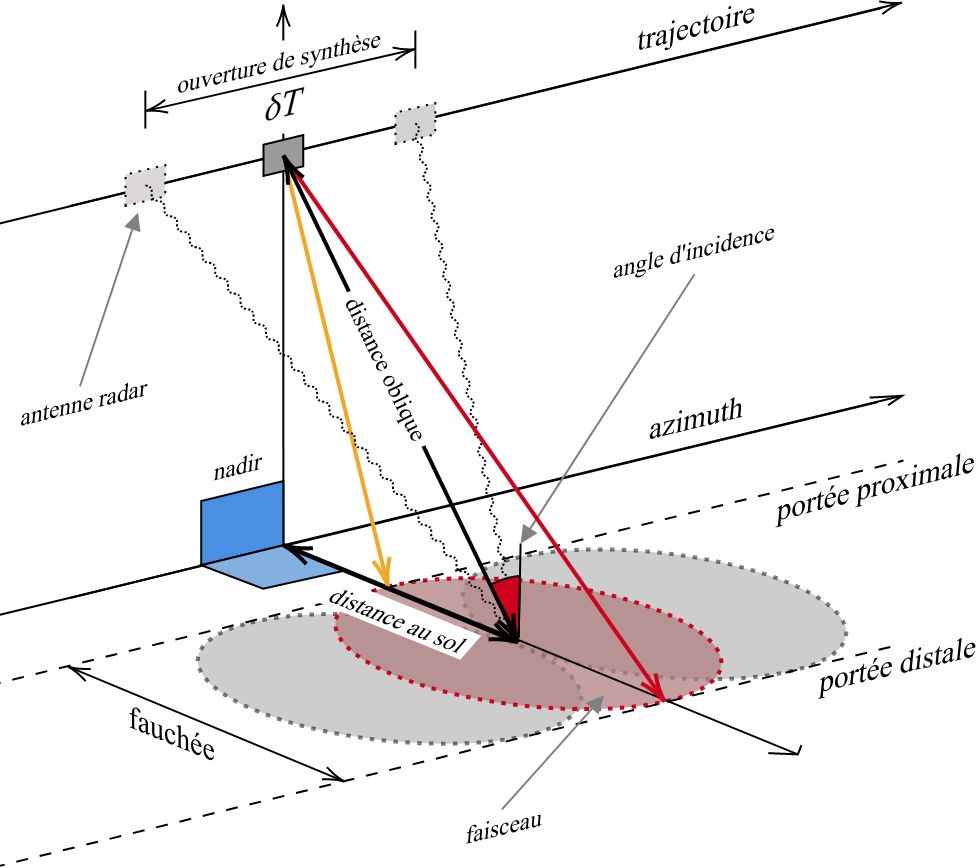
\includegraphics[width=0.85 \linewidth]{figures/sar-geom-diagram.jpg}
   \centering
\caption
{\small Géométrie de l'acquisition des images \acrsar et \acrpolsarns.}
  \label{fig:sar-geoms-diagram}
\end{figure}

En mode transmission,  les capteurs \acrpolsar émettent des ondes polarisées linéairement selon des axes orthogonaux: soit H pour la polarisation horizontale et V pour la polarisation verticale.  En mode réception, ils mesurent la rétrodiffusion polarisée horizontalement (H) et verticalement (V) (Fig. ~\ref{fig:polsar-acquisition-diagram}). Une image \acrpolsar est formée en mesurant l’énergie rétrodiffusée selon les 4 combinaisons réception-transmission possibles, soient $HH$, $HV$, $HV$, $VV$ (Fig. ~\ref{fig:polsar-bands-diagram}).


\begin{figure}[!htbp] 
  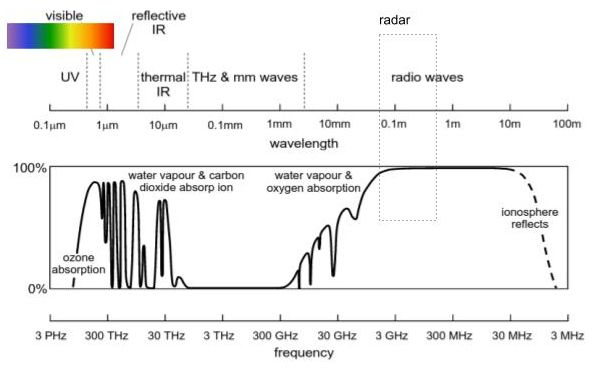
\includegraphics[width=0.80 \linewidth]{figures/atm-windows-diagram.jpg} 
   \centering
\caption
{\small Le spectre électromagnétique et la transmittance de l'atmosphère entre l'espace et la terre.  L'atmosphère est transparente dans le domaine des hyperfréquences (3GHz à 300 MHz). \cite{Richards:2009:RSI:1816335} }
  \label{fig:atm-windows-diagram}
\end{figure}


\begin{figure}[!htbp] 
  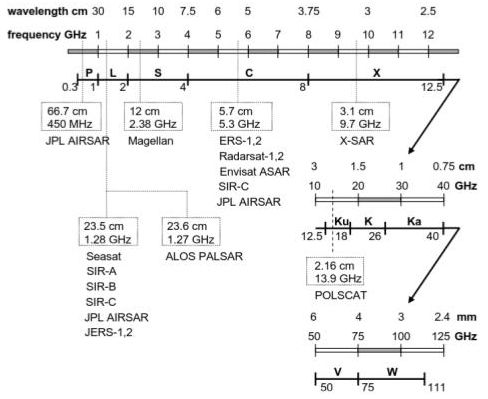
\includegraphics[width=0.80 \linewidth]{figures/sar-bands-diagram.jpg}
   \centering
\caption
{\small Les bandes utilisées par les capteurs \acrsar et \acrpolsarns.  \cite{Richards:2009:RSI:1816335}}
  \label{fig:sar-bands-diagram}
\end{figure}

\begin{figure}[!htbp] 
  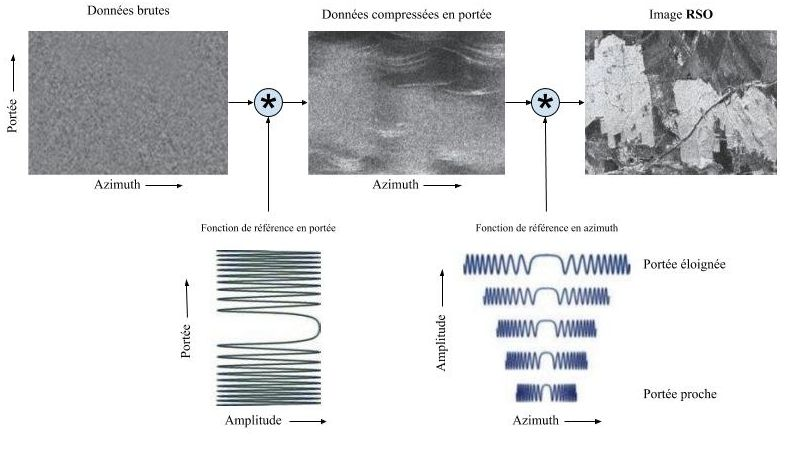
\includegraphics[width=1.0 \linewidth]{figures/sar-processing-diagram.jpg}
   \centering
\caption
{\small Résumé du procédé de la formation des images \acrsar à partir de la donnée brute (adapté de \cite{SarTutorial2013}). } 
  \label{fig:sar-processing-diagram}
\end{figure}

\begin{figure}[!htbp] 
  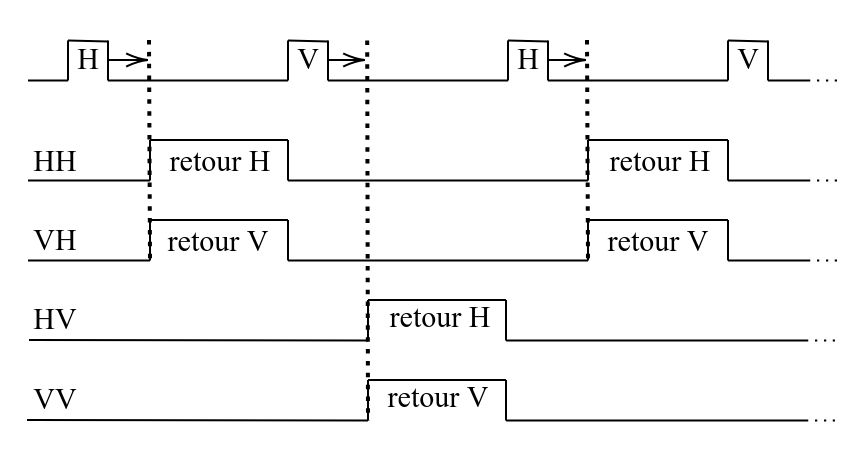
\includegraphics[width=0.80 \linewidth]{figures/polsar-acquisition-diagram.jpg}
   \centering
\caption
{\small La séquence des impulsions transmise et reçue par l'antenne d'un capteur $\acrpolsarns$.  Dans le cas des plateformes satellitaires, la séquence transmission/réception n'est pas nécessairement immédiate.}
  \label{fig:polsar-acquisition-diagram}
\end{figure}

%\figureQuadpolBandsExample{!htbp}{0.45}

\begin{figure}[!htbp] 
\centering
\subcaptionbox[]{Polarisation HH\label{fig:Polarisation-HH}}
{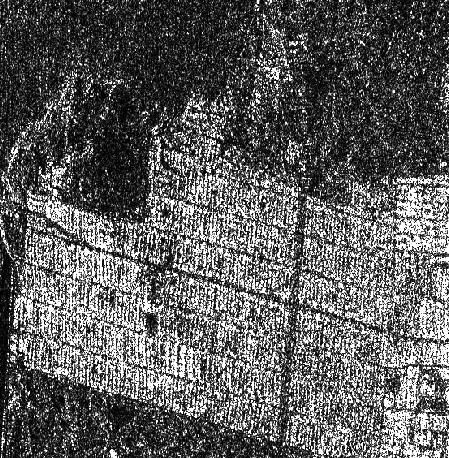
\includegraphics[width=0.45 \linewidth]{figures/Chap2/polsar_bands_sf/RS2-SLC-FQ9-ASC-09-Apr-2008_02_Intensity_HH-diagram.jpg}}
\subcaptionbox[]{Polarisation HV\label{fig:Polarisation-HV}}
{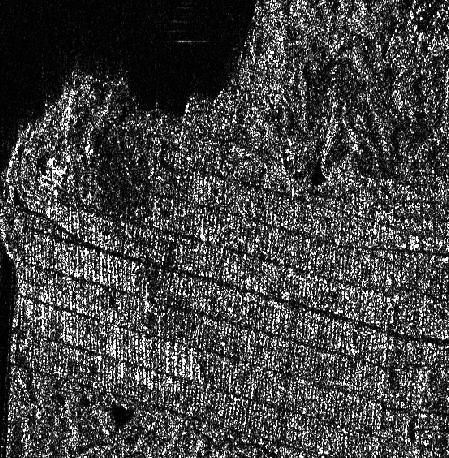
\includegraphics[width=0.45  \linewidth]{figures/Chap2/polsar_bands_sf/RS2-SLC-FQ9-ASC-09-Apr-2008_02_Intensity_HV-diagram.jpg}}
\subcaptionbox[]{Polarisation VH\label{fig:Polarisation-VH}}
{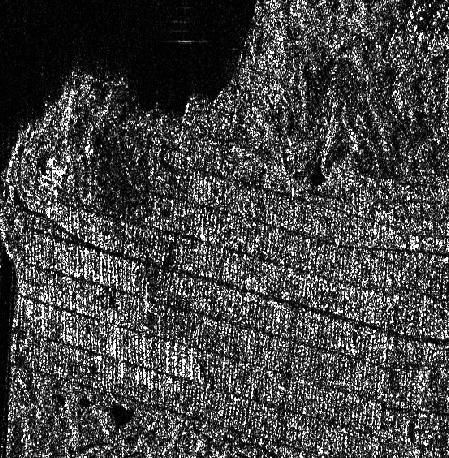
\includegraphics[width=0.45  \linewidth]{figures/Chap2/polsar_bands_sf/RS2-SLC-FQ9-ASC-09-Apr-2008_02_Intensity_VH-diagram.jpg}}
\subcaptionbox[]{Polarisation VV\label{fig:Polarisation-VV}}
{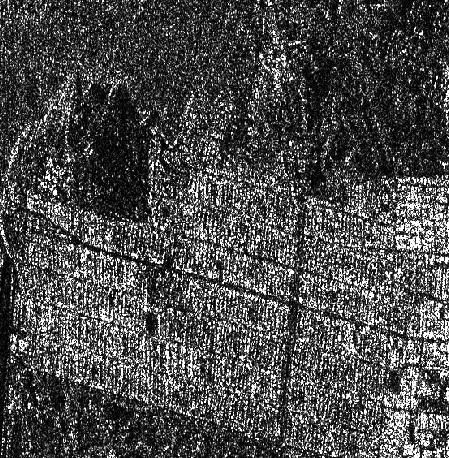
\includegraphics[width=0.45  \linewidth]{figures/Chap2/polsar_bands_sf/RS2-SLC-FQ9-ASC-09-Apr-2008_02_Intensity_VV-diagram.jpg}}
 \caption
        {\small Les quatre bandes polarimétriques d'une image en QuadPol RADARSAT-2 (San Francisco, Californie)} 
        \label{fig:polsar-bands-diagram}
\end{figure}

\subsection{La polarimétrie RSO}

La polarimétrie \acrsar étudie les propriétés d’une cible en fonction des caractéristiques du comportement de l’onde électromagnétique (\acrcroens) rétrodiffusée par celle-ci.  Les facteurs qui affectent la mesure de l’énergie rétrodiffusée au niveau du capteur sont: la fréquence de l’onde, la polarisation, l’angle d’incidence et l’orientation de la visée. Les facteurs qui influencent la mesure au niveau de la cible sont: les propriétés géométriques (structure, orientation) et géophysiques (rugosité, humidité du sol, conductivité du médium).

De manière générale, la modélisation des interactions de l’\acrcroe polarisée avec un milieu peut être décrite par la projection du champ électrique $\Vec{E}$ sur un plan perpendiculaire à la direction de propagation de celle-ci.  Le vecteur du champ $\Vec{E}$ dessine ainsi une ellipse en fonction du temps: l’ellipse de polarisation.  Cette dernière peut à son tour être représentée par une combinaison linéaire de deux états de polarisation d’amplitude $(E_x, E_y)$  avec la base des vecteurs d’états orthogonaux $\{\Vec{e}_x, \Vec{e}_y\}$

\begin{equation}
    \Vec{E}  = E_x \Vec{e}_x + E_y \Vec{e}_y
    \label{eq:E}
\end{equation}

\vspace{10pt}

Cette formulation (Eq. \ref{eq:E}) peut se réécrire selon le vecteur de Jones en coordonnées polaires

\begin{equation}
    E_{x_y}  = \begin{bmatrix} E_x \\ E_y \end{bmatrix} = \begin{bmatrix} |E_x|e^{i {\phi_x}}  \\ |E_y|e^{i {\phi_y}}\end{bmatrix}
    \label{eq:E2}
\end{equation}

\vspace{10pt}

Dans notre cas, les états représentés par la base $\{\Vec{e}_x, \Vec{e}_y\}$ sont assimilés aux états de polarisation linéaire (H, V).  Nous ne décrirons pas le cas de la polarisation circulaire.  Nous pouvons définir la matrice $\matscat$ comme la matrice de rétrodiffusion qui décrit la façon dont l’\acrcroe transmise a été dépolarisée par les cibles au sol et mesurée par le capteur:

\begin{equation}
\matscat=\begin{bmatrix} S_{HH} &  S_{HV} \\ S_{VH} &  S_{VV}\end{bmatrix}
\end{equation}

\vspace{10pt}

Le vecteur de Jones se formule en tenant compte de la matrice de rétrodiffusion comme suit:

\begin{equation}
\begin{bmatrix} E_x \\ E_y \end{bmatrix}_{reception} = \frac{e^{ikr}}{kr} \matscat=\begin{bmatrix} S_{HH} &  S_{HV} \\ S_{VH} &  S_{VV}\end{bmatrix} = \begin{bmatrix} E_x \\ E_y \end{bmatrix}_{transmission}
\end{equation}

\vspace{10pt}

 Les quatre coefficients de la matrice  $\matscat$ sont des nombres qui enregistrent l'amplitude et la phase de l'onde sous forme complexe. Les éléments $S_{HH}$ et $S_{VV}$ mesurent la puissance du retour de la polarisation dans le même axe, tandis que les éléments $S_{HV}$ et $S_{VH}$ mesurent cette puissance dans les axes croisés. Dans le cas mono-statique, où l’antenne de réception et de transmission sont les mêmes, la matrice est aussi nommée matrice de Sinclair et les coefficients $S_{HV}$ et $S_{VH}$ sont égaux. 
 
%  Le \itspan de la matrice \matscat mesure la puissance totale de la rétrodiffusion. Il est donné par la somme des carrés des éléments de la matrice \matscat:
 
%  \begin{equation}
%     \itspanns = \simplevmatrixnorm{S_{HH}}^2 +\simplevmatrixnorm{S_{HV}}^2 +\simplevmatrixnorm{S_{VH}}^2 
%     +\simplevmatrixnorm{S_{VV}}^2 = Tr(\matscat \matscat^H)
%  \end{equation} 
 
%  qui se réduit dans le cas réciproque à
 
%   \begin{equation}
%     \itspanns = \simplevmatrixnorm{S_{HH}}^2 + 2\simplevmatrixnorm{S_{HV}}^2 
%     +\simplevmatrixnorm{S_{VV}}^2 
%  \end{equation}
 
Les cibles d’origine anthropique sont stationnaires et leurs propriétés polarimétriques sont souvent caractérisées par un mécanisme de rétrodiffusion unique.  Dans ce cas,  l’observation d’une seule matrice de Sinclair permet de caractériser la cible.  Cependant dans la plupart des observations, les cibles naturelles sont des cibles étendues et leurs propriétés polarimétriques sont généralement hétérogènes.   Dans ce cas, la matrice de Sinclair décrit plutôt la superposition d'un ensemble de matrices de diffusion représentant les différents diffuseurs dans la cellule de résolution.  Afin de bien décrire les caractéristiques de rétrodiffusion polarimétrique des cibles étendues on utilise plutôt une analyse statistique de second ordre. Le formalisme le plus courant pour caractériser complètement les diffuseurs distribués est l'emploi de la matrice $3\times3$ de cohérence $\matcoh$ (ou de covariance $\matcov$).  %Elles permettent de mesurer la corrélation entre les composantes du champ électrique sur un intervalle de temps $t$ contrairement à la matrice \matscat. 
Les matrices $\matcoh$ ou $\matcov$ permettent de calculer une moyenne d’ensemble sur
plusieurs cellules de résolution (pixels) contiguës pour la réduction du chatoiement des
images en QuadPol.

On obtient la matrice de covariance $\matcov$ à partir de la matrice $\matscat$ en représentant cette dernière sous la forme du vecteur lexicographique $\Vec{k}_C$:
 \begin{equation}
 \Vec{k}_C = \begin{bmatrix} S_{HH} \\ \sqrt{2}S_{HV}  \\  S_{HH}\end{bmatrix}
 \end{equation}
 
et la matrice de covariance  $\matcov$ nous est donnée par la moyenne des produits:
 \begin{equation}
\matcov = \frac{1}{L_n} \sum_{i=1}^{L}(\Vec{k}_{iC} \cdot \Vec{k}_{iC}^{H})
 \end{equation}
 
 \vspace{10pt}
 
 où l’opération Hermitienne H est définie comme le conjugué transposé du vecteur complexe $\Vec{k}_{C}$ et $L_n$ exprime le nombre de vues sur lequel la matrice est moyennée et l’opérateur $\langle \cdot \rangle$ résume l’opération de moyennage sur un voisinage.  

\begin{equation}
\matcov = \begin{bmatrix} 
\bracket{S_{hh} S_{hh}^*} & \bracket{\sqrt{2} S_{hh} S_{hv}^*} & \bracket{S_{hh} S_{vv}^*} \\
 \bracket{\sqrt{2} S_{hv} S_{hh}^*} & \bracket{2 S_{hv} S_{hv}^*} & \bracket{\sqrt{2} S_{hv} S_{vv}^*} \\
 \bracket{S_{vv} S_{hh}^*} & \bracket{\sqrt{2} S_{vv} S_{hv}^*} & \bracket{S_{vv} S_{vv}^*}
\end{bmatrix}
\end{equation}

\vspace{10pt}

 De manière similaire la matrice de cohérence  $\matcoh$ est obtenue à partir de la représention  de la matrice $\matscat$ sous la forme  du vecteur de Pauli :
  \begin{equation}
 \Vec{k}_T =\frac{1}{\sqrt{2}} \begin{bmatrix} S_{HH}+S_{VV} \\ S_{VV}-S_{HH} \\  2S_{HV}\end{bmatrix}
 \end{equation}
et par le produit suivant:
  \begin{equation}
\matcoh = \frac{1}{L_n} \sum_{i=1}^{L}(\Vec{k}_{iT} \cdot \Vec{k}_{iT}^{H})
 \end{equation}
 \begin{equation}
\matcoh = \frac{1}{2} \begin{bmatrix} 
\bracket{ {|S_{hh} + S_{vv}|}^2} & \bracket{(S_{hh} + S_{vv})(S_{hh} - S_{vv})^*} & \bracket{2(S_{hh}+S_{vv})S_{hv}^*} \\
\bracket{(S_{hh} - S_{vv})(S_{hh} + S_{vv})^*} & \bracket{ {|S_{hh} - S_{vv}|}^2} & \bracket{2(S_{hh}-S_{vv})S_{hv}^*} \\
 \bracket{2S_{hv}(S_{hh}+S_{vv})^*} & \bracket{2S_{hv}(S_{hh}-S_{vv})^*} & 4\bracket{{|S_{hv}|}^2}
\end{bmatrix}
\end{equation}

\vspace{10pt}

 Les matrices $\matcoh$ et $\matcov$ sont des matrices Hermitiennes définies positives de rang 3.  Elles partagent les mêmes valeurs propres positives, ce qui implique que leurs traces sont égales:
\begin{equation}
    Tr(\matcoh) = Tr(\matcov) = \itspanns
\end{equation}  

\vspace{10pt}

où le \itspan est la mesure de la puissance totale de la rétrodiffusion. Par contre leurs vecteurs propres orthogonaux respectifs sont différents.
 
 Les matrices $\matcoh$ et $\matcov$  sont similaires et interchangeables sous une transformation linéaire $\begin{bmatrix}U_3\end{bmatrix}$.
  \begin{equation}
  \Vec{k}_T = \frac{1}{\sqrt{2}} 
 \begin{bmatrix}
  +1 & 0 & +1 \\
  +1 & 0 &-1 \\
  0 & \sqrt{2} & 0
  \end{bmatrix} \Vec{k}_C \iff  \Vec{k}_T = \simplematrix{U_3}  \Vec{k}_C
  \end{equation}
  Nous avons donc:
\begin{equation}
    \simplematrix{T_3}= \simplematrix{U_3}   \simplematrix{C_3}   \simplematrix{U_3}^{-1}
\end{equation}

\vspace{10pt}

 Elles génèrent des résultats équivalents et contiennent la même information polarimétrique.  Ainsi le choix de la représentation (\matcoh ou \matcov) des données est arbitraire.  Cependant pour la suite des travaux,  nous utiliserons seulement la représentation en matrice de cohérence $\matcoh$ des images en QuadPol car elle présente l’avantage de facilement visualiser la décomposition de Pauli à partir des termes diagonaux de la matrice.
 
 A noter que la conséquence du moyennage sur un voisinage est la dégradation de l'information spatiale lorsque l'on utilise les matrices \matcoh et \matcov comme outils d'analyse. 
 
\subsection{Le chatoiement des images RSO et RSOPOL} \label{sec:speckle}

A cause de la nature cohérente du signal \acrsarns, les mesures de la matrice de Sinclair sont affectées par le bruit de chatoiement (\textit{speckle}) et par la même occurence les matrices \matcoh et \matcov.  C'est ce qui donne un aspect sel et poivre sur chacun des canaux des images en QuadPol (Fig. \ref{fig:polsar-bands-diagram}).  Le chatoiement est le résultat de la sommation cohérente de plusieurs échos radars en provenance des diffuseurs élémentaires d’une cellule de résolution. La Figure ~\ref{fig:speckle-diagram} donne une illustration du phénomène. Si nous supposons que la cellule contient $N$ diffuseurs, chacun diffusant un signal complexe $a_i e^{j\phi_i}$ alors la
mise "bout à bout" de ces contributions dans le plan complexe, mesure la réponse
totale du pixel, en amplitude et en phase.
\begin{equation}
A e^{j\Phi} = \sum_{i=1}^{N}(a_i e^{j\phi_i}) = \sum_{i=1}^{N}(a_i (x_i+jy_i)) = A(X+jY)
\end{equation}
La distribution aléatoire des diffuseurs fait en sorte que les ondes rétrodiffusées ne sont plus nécessairement en phase. Il arrive donc que la sommation des échos produise une forte rétrodiffusion qui n'est pas nécessairement en relation avec la vraie réflectivité. On parlera d’interférences constructives.  Dans le cas contraire, le cas d’interférences destructives, le signal sera moindre que le vrai signal.

%C'est ce qui donne l'aspect sel et poivre sur les régions homogènes. 

\begin{figure}[!htbp] 
  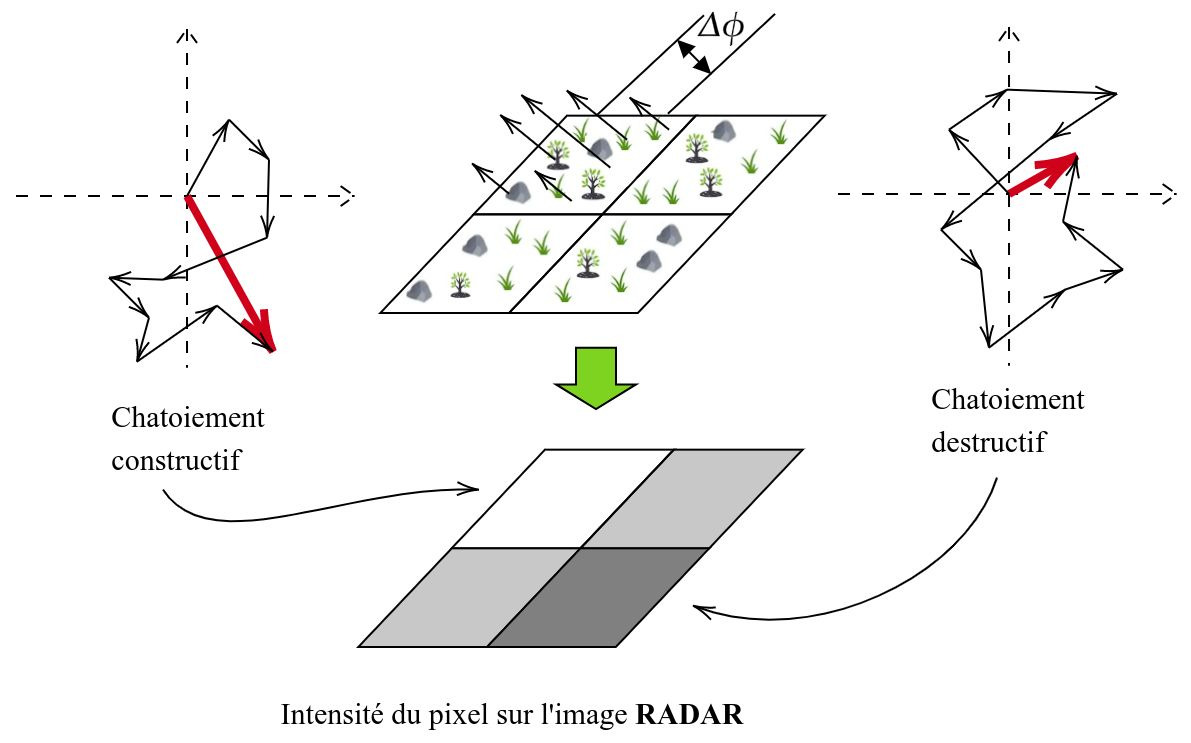
\includegraphics[width=1.0 \linewidth]{figures/speckle-diagram.jpg}
   \centering
        \caption
        {\small Illustration du mécanisme de formation du chatoiement.}
  \label{fig:speckle-diagram}
\end{figure}

Le chatoiement est modélisé mathématiquement comme un bruit aléatoire multiplicatif sous l'hypothèse du "chatoiement pleinement développé" \cite{Goodman76}. Cette hypothèse impose que le chatoiement soit indépendant du type de surface observée, que les diffuseurs contenus dans une cellule de résolution soient en grand nombre et statistiquement indépendants les uns des autres et que leurs phases soient distribuées uniformément dans l’intervalle $[-\pi, \pi]$ sur les régions homogènes. Sous ces conditions, en vertu du théorème de la limite centrale, les composantes réelles $X$ et imaginaires $Y$ du signal peuvent être représentées comme  des variables aléatoires indépendantes suivant une loi normale centrée sur zéro et de même écart-type $\sigma$:

\begin{equation}
  \left\{
    \begin{aligned}
        p(X=x) = \frac{1}{\sigma\cdot\sqrt{2\cdot\pi}}\cdot exp(-\frac{x^2}{2\cdot\sigma^2})  \\
        p(Y=y) = \frac{1}{\sigma\cdot\sqrt{2\cdot\pi}}\cdot exp(-\frac{y^2}{2\cdot\sigma^2})
    \end{aligned}
  \right.
\end{equation}
% avec 
% \begin{equation}
%   \left\{
%     \begin{aligned}
%         E (x_i) = E (y_i) = 0 \\
%         E (x_i\cdot x_k) = E (y_i\cdot y_k)  \\
%         E (y_i\cdot x_k) = -E (x_i\cdot y_k) \\
%         E (x_i\cdot y_i ) = 0
%     \end{aligned}
%   \right.
% \end{equation}

La densité de probabilité de l'intensité $(I=X^2+Y^2)$ du chatoiement dans les régions homogènes est décrite par une loi exponentielle dans le cas des données une vue et d'une loi Chi-carré dans le cas des données multivues donnée par:

\begin{equation}
    P(I) =\frac{L_n^{L_n}\cdot I^{L_n-1}}{(N-1)! \cdot \sigma^{2N}} exp(-\frac{L_n \cdot I}{\sigma^2})
\end{equation}

\vspace{10pt}

où $L_N$ exprime le nombre de vues. La Figure  ~\ref{fig:gamma-diagram} présente la distribution Chi-carré en fonction de différentes valeurs de $L_n$. Dans le cas des images une vue, $L_n$ est égal à 1 et la distribution est exponentielle. 

\begin{figure}[!htbp] 
  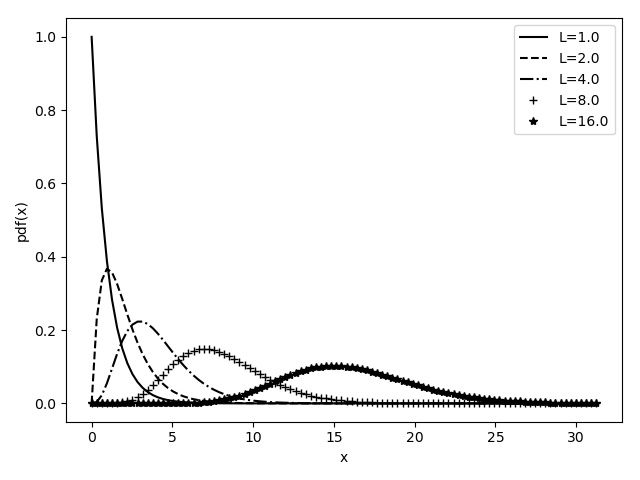
\includegraphics[width=0.85 \linewidth]{figures/gamma-pdf-diagram.jpg}
   \centering
        \caption
        {\small Distribution des données \acrsar en fonction du nombre de vues $L_n$}
  \label{fig:gamma-diagram}
\end{figure}

Dans le cas de l'imagerie polarimétrique, le vecteur de rétrodiffusion $\Vec{k}_C$ peut être décrit comme une variable aléatoire suivant une loi normale complexe circulaire multidimensionnelle centrée sur zéro:

\begin{equation}
p(\Vec{K}_C=\Vec{k}_C) = \frac{1}{\pi^3\cdot\simplevmatrixnorm{\boldsymbol{C}}} exp(-\Vec{k}_{C}^{H}\cdot\boldsymbol{C}^{-1}\cdot\Vec{k}_{C})
\end{equation}

\vspace{10pt}

où $\simplevmatrixnorm{\boldsymbol{C}}$ est le déterminant de la matrice de covariance polarimétrique. L'estimé de la matrice de covariance ($\boldsymbol{Z}$) dans le cas multivues est donné par le moyenne des matrices de covariance dans un voisinage:
\begin{equation}
\boldsymbol{Z}=\frac{1}{L_n} \sum_{i=1}^{L}{\boldsymbol{C}_i}
\end{equation}

\vspace{10pt}

Dans ce cas, la matrice $\boldsymbol{Z}$ peut être décrite comme une variable aléatoire suivant une distribution de Wishart avec la densité de probabilité:

\begin{equation}
    P(Z) =  \frac{L^{3L} \simplevmatrixnorm{\boldsymbol{Z}^{L-3}}  }{\simplevmatrixnorm{\boldsymbol{C}}^L\pi^3 \prod_{i=1}^{3} \Gamma(L-i+1)} exp(-L\cdot Tr(\boldsymbol{C}^{-1} \cdot \boldsymbol{Z}))
\end{equation}

\vspace{10pt}

Nous pourrons par la suite utiliser cette connaissance sur la distribution statistique du chatoiement pour simuler des données polarimétriques une-vue. Par contre, notons que dans la pratique, les conditions du "chatoiement pleinement développé" ne sont pas toujours respectées si bien que la description du chatoiement se rapproche plus d'un modèle de texture. Dans ce cas, le chatoiement sera dépendant du type de surface et peut même aider à l’interprétation de la scène.  
 
 \subsection{La décomposition polarimétrique} \label{section:decomposition_polarimetric}
 
 L’objectif principal d’une décomposition polarimétrique est d'exprimer la matrice de diffusion $\begin{bmatrix} S_2 \end{bmatrix}$ selon des mécanismes polarimétriques  canoniques dans le cas d’une décomposition cohérente ou selon des descripteurs plus simples de la matrice  $\matcov$  ou de la matrice  $\matcoh$  dans le cas d’une décomposition incohérente. Dans le cas des cibles cohérentes, on privilégie les méthodes de décomposition cohérente, par exemples les approches de Pauli, Krogager \cite{Krogager1990}, Cameron \cite{Cameron1996}.  Dans le cas des cibles étendues, on utilisera plutôt les approches de décomposition incohérente selon Freeman \cite{Freeman1998}, Huynen ou Cloude-Pottier \cite{Cloude1996}.
 
L'approche que nous utiliserons au cours de l'évaluation des résultats est la décomposition polarimétrique basée sur les valeurs propres de la matrice de cohérence $\matcoh$ de Cloude et Pottier \cite{Cloude1997}.  Elle consiste à exprimer la matrice $\matcov$  sous la forme:

\begin{equation}
    \matcoh=\simplematrix{U_3} \simplematrix{\Lambda_3} \simplematrix{U_3}^H = \sum_{k=1}^{3} \lambda_k \Vec{u}_k\cdot \Vec{u}_k^H
\end{equation}

\vspace{10pt}

où $\simplematrix{U_3}$ représente la matrice des vecteurs propres $\Vec{u}_k$ et $\simplematrix{\Lambda_3}$ représente la matrice diagonale des valeurs propres $\lambda_k$. Les vecteurs propres de la décomposition sont donnés par 

\begin{equation}
    \Vec{u}_k=[\cos{\alpha_k}, 
    \sin{\alpha_k} \sin{\beta_k} e^{j\delta_k}, 
    \sin{\alpha_k} \sin{\beta_k} e^{j\gamma_k} ]^T 
\end{equation}

\vspace{10pt}

Cette décomposition peut être interprétée comme la somme de trois matrices de cohérence $\matcoh_k = \Vec{u}_k \cdot  \Vec{u}_k^H$ (avec $k=1,2,3$)  non corrélées décrivant les caractéristiques de la cible.
A partir des paramètres principaux $\lambda_k$ et $\alpha_k$, on peut calculer les trois paramètres de la décomposition $H/A/\Bar{\alpha}$:

L’entropie $H$ permet de quantifier le caractère aléatoire du processus de diffusion lié à la réponse polarimétrique. La valeur de l'entropie est égale à la somme logarithmique des valeurs propres normalisées de \matcoh:

\begin{equation}  
    H = \sum_{k=1}^{3}p_k \log_3 p_k
\end{equation}

avec 

\begin{equation}  
    p_k = \frac{\lambda_k}{\sum_{k=1}^{3}\lambda_k}
\end{equation}

\vspace{10pt}

$H$ est comprise entre 0 et 1. Les cas extrêmes rencontrés sont les mécanismes de rétrodiffusion non dépolarisants où $H = 0$, indiquant la présence d'un diffuseur dominant, et les mécanismes de rétrodiffusion totalement dépolarisants, où $H = 1$, suggérant la présence de plusieurs types de diffuseur de force égale.

L’anisotropie $A$ varie aussi entre 0 et 1. Elle permet de mesurer l'importance relative des diffuseurs secondaires et apporte une information complémentaire à $H$ dans le cas où l’entropie polarimétrique possèderait une valeur moyenne.  L'anisotropie est calculée comme suit:
\begin{equation}  
    A = \frac{\lambda_2 -\lambda_3 }{\lambda_2 +\lambda_3}
\end{equation}

\vspace{10pt}

L’angle  $\midpoint{\alpha}$ décrit physiquement le mécanisme de diffusion et varie entre $0^{\circ}$ et $90^{\circ}$.

\begin{equation}  
    \midpoint{\alpha} =  \sum_{k=1}^{3}p_k \cdot \alpha_k
\end{equation}

\vspace{10pt}

 Pour des valeurs proches de $0^{\circ}$, l’angle $\midpoint{\alpha}$  indique la présence de diffuseurs surfaciques. Si les
valeurs sont proches de  $45^{\circ}$ alors elle indique une diffusion volumétrique. Et pour des
valeurs qui tendent vers  $90^{\circ}$, le mécanisme de rétrodiffusion s'apparente à celui d’un dièdre, à double rebond.
\begin{figure}[!htbp] 
  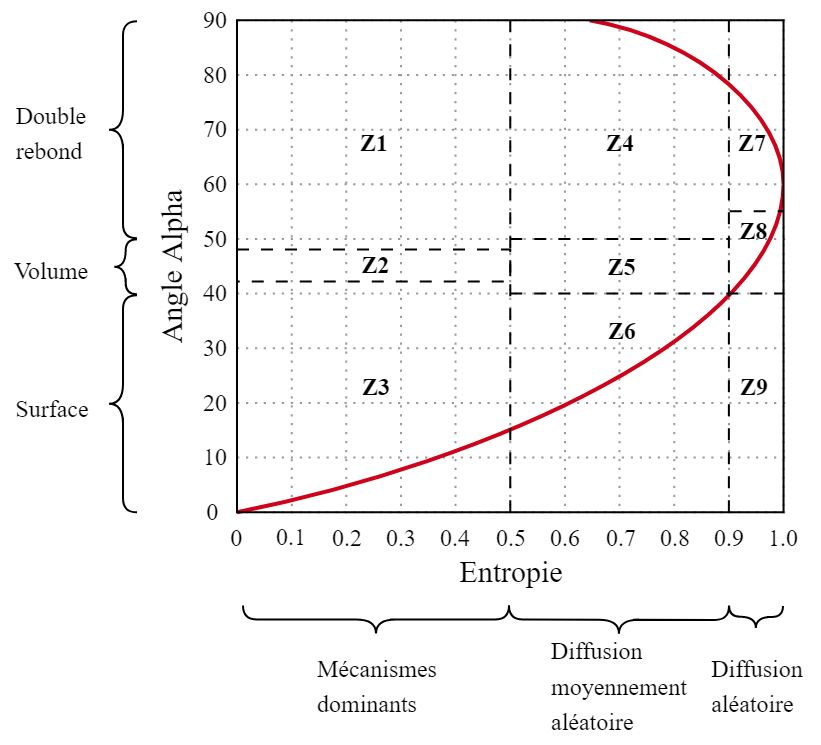
\includegraphics[width=1.0 \linewidth]{figures/haalpha-diagram.jpg}
   \centering
        \caption
        {\small Diagramme $H/\midpoint{\alpha}$ avec les régions qui définissent les limites des classes de diffuseurs de Cloude-Pottier}
  \label{fig:haalpha-diagram}
\end{figure}

La Figure ~\ref{fig:haalpha-diagram} montre le diagramme $H/\midpoint{\alpha}$. La courbe (rouge) donne pour chaque
valeur de l’entropie $H$ les bornes minimales et maximales pour $\midpoint{\alpha}$.  En fonction de l'entropie $H$, on peut séparer le diagramme en trois grandes zones qui à leur tour peuvent être raffinées en fonction de l'angle $\midpoint{\alpha}$:



\begin{enumerate}
    \item les zones de diffusion de faible entropie pour lesquelles un seul mécanisme de
diffusion prédomine:
    \begin{enumerate}
    \item  $\boldsymbol{Z3}$  (Surfaces de Bragg):  $\midpoint{\alpha}$ est inférieur à $\pi/4$, ce qui correspond à une simple diffusion par une surface (sans mécanisme introduisant une rotation de phase de $\pi$ entre HH et VV). En pratique, tous les mécanismes décrits par un nombre impair de diffusions appartiennent à cette classe: par exemple les surfaces d'eau.
    
    \item $\boldsymbol{Z1}$ (Réflecteurs dièdraux):  $\midpoint{\alpha}$ est supérieur à $\pi/4$ et inférieur à $\pi/2$, ce qui correspond à une diffusion double. En pratique, tous les mécanismes décrits par un nombre pair de diffusions appartiennent à cette classe.
    \item $\boldsymbol{Z2}$ (Dipôles):  $\midpoint{\alpha}$ est proche de $\pi/4$, le mécanisme proposé est une diffusion par des dipôles. Ce mécanisme est fortement corrélé avec un déséquilibre prononcé en amplitude entre HH et VV
    \end{enumerate}
    
    \item les zones de diffusion d'entropie moyenne (entre 0.5 et 0.9)
    
     \begin{enumerate}
    \item  $\boldsymbol{Z6}$  (Surfaces aléatoires): $\midpoint{\alpha}$ est faible, on a affaire à des mécanismes de diffusion simple avec des effets liés à la rugosité de la surface.
     \item  $\boldsymbol{Z4}$  (Double réflections):  $\midpoint{\alpha}$ est supérieur à $\pi/4$, on a des effets de diffusion multiple (par exemple, diffusion volumique dans la canopée).
      \item  $\boldsymbol{Z5}$  (Particules anisotropiques):  $\midpoint{\alpha}$ est proche de $\pi/4$ , ce qui peut s’expliquer par une certaine corrélation entre l’orientation des diffuseurs.

      \end{enumerate}
      
      
     \item les zones de diffusion de forte entropie
     \begin{enumerate}
       \item  $\boldsymbol{Z9}$ (Zone impossible):  $\midpoint{\alpha}$ est faible, ce qui correspond à des valeurs de $\midpoint{\alpha}$ supérieures à la borne supérieure, ne peut se caractériser par cette approche.

     \item  $\boldsymbol{Z7}$  (Structures complexes):   cette zone correspond à des diffusion multiples, telles que l’on peut les observer en forêts.
      \item  $\boldsymbol{Z8}$ (Diffuseurs anisotropiques aléatoires): cette zone correspond donc à de la diffusion volumique par un nuage de
particules de type aiguille.

      \end{enumerate}
    
\end{enumerate}


À noter que les limites sont arbitraires et dépendent de l'étalonnage du radar, du bruit minimum des observations et de la variance des estimations des paramètres.

\newpage
\section{Les réseaux neuronaux artificiel et l'apprentissage automatique}
Les réseaux de neurones sont des constructions abstraites qui simulent l’activité des réseaux de neurones biologiques élémentaires. Ils sont utilisés en apprentissage automatique pour construire des modèles à partir de données existantes dans le but d’effectuer des prédictions sur de nouvelles données soit à l’aide de classification, dans le cas discret, ou  de régression, dans le cas continu. 
La topologie des réseaux neuronaux est diversifiée et il est difficile de répertorier toutes les variétés existantes et leurs applications.  Liu et al. \cite{Liu2017ASO} propose une revue des architectures les plus utilisées en apprentissage machine profond (comme le \acrconvnetns). Van Veen \cite{VanVeen2016} fait une revue exhaustive des topologies et des différents types de neurones que l’on retrouve actuellement dans la littérature.  On y dénombre pas moins d'une trentaine d'architectures neuronales, mais quelques architectures importantes sont manquantes comme le UNet (Ronnenberg \cite{Ronneberger2015UNetCN}).  Dans le cadre de ce mémoire nous concentrons notre attention sur les \acrconvnetns.

\subsection{Les neurones artificiels}

Le premier modèle du neurone artificiel a été présenté par McCulloch et Pits \cite{McCulloch1943}. Un neurone artificiel est un modèle mathématique d'un neurone biologique.  Il possède généralement plusieurs entrées et une sortie qui correspondent par analogie aux dendrites et au cône d'émergence du neurone biologique. Les actions excitatrices et inhibitrices des synapses sont modélisées par les poids (paramètres) associés aux entrées. Les valeurs numériques de ces poids sont ajustées lors de la  phase d'apprentissage. Dans sa version la plus simple, un neurone artificiel calcule la somme pondérée des entrées reçues, puis applique à cette valeur une fonction d'activation, généralement non linéaire. La valeur finale obtenue est la sortie du neurone. 


\begin{figure}[!htbp] 
  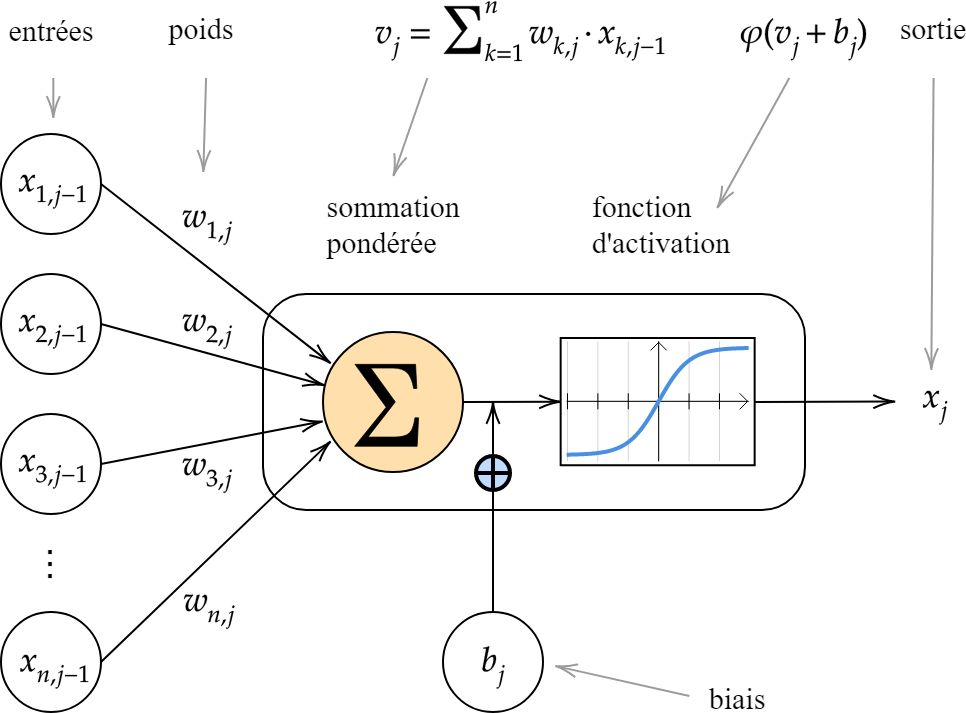
\includegraphics[width=0.75\linewidth]{figures/Chap2/neurones-artificiels-diagram.jpg}
   \centering
    \caption{\small Structure d'un neurone artificiel. Le neurone calcule la somme de ses entrées puis cette valeur passe par la fonction d'activation pour produire sa sortie.}
  \label{fig:neurones_artificiels}
\end{figure}

 La Figure ~\ref{fig:neurones_artificiels} illustre un exemple de base d'un modèle non-linéaire d'un neurone, où $x_{1,j-1}$, $x_{2,j-1}$, $x_{3,j-1}$, $\dots$ $x_{n,j-1}$ sont les signaux d'entrée de la couche $j-1$; $w_{1,j}$, $w_{2,j}$, $w_{3,j}$, $\dots$ $w_{n,j}$ sont les poids synaptiques de la couche $j$; $v_j$ est la valeur de pré-activation qui correspond à la combinaison linéaire des signaux d'entrées; $\varphi(\cdot)$ est une fonction d'activation non-linéaire telle que la fonction tangente hyperbolique, et $x_j$ est la sortie de la couche $j$. Le biais $b_j$ est sommé avec la valeur de pré-activation ce qui vaut à l'application d'une transformation affine pour calculer la sortie.
 
 Considérant que les poids peuvent être condensés en une matrice \textbf{W} où chaque colonne contient les paramètres menant à un neurone, que les entrées et les biais peuvent être représentés par des vecteurs, le calcul sur une couche donnée peut s'exprimer simplement par une transformation affine suivie d'une fonction non linéaire:
 
 \begin{equation}
     h = \varphi_i(W^\intercal x + b)
     \label{eq:h_matricielle}
 \end{equation}

\subsection{Les réseaux de neurones artificiels}

Un réseau de neurones peut être vu comme un assemblage de neurones connectés ensembles suivant une loi de connectivité que l'on définit. Le réseau peut être décrit par un graphe où les noeuds sont les neurones et les arêtes sont les connexions entre les neurones. Dans le cas des réseaux neuronaux acycliques (\textit{feed-forward}), ils propagent l’entrée du réseau vers les couches suivantes sans jamais revenir en arrière. Ils sont assemblés comme une composition de fonctions.

\begin{equation}
    y = f(x) =  \varphi(w_j \dots \varphi(w_2 \cdot \varphi(w_1 \cdot x+b_1)+b_2 \dots + b_j)
\end{equation}

Un exemple classique est le réseau perceptron multicouche (\acrmlpns). Les neurones sont combinés par couche tel que présenté par la Figure ~\ref{fig:reseau_neurones_artificiels}. Il n'y a pas de connexion entre neurones d'une même couche et les connexions sont établis qu'avec les neurones des couches en aval. Habituellement, chaque neurone d'une couche est connecté à tous les neurones de la couche suivante.  Par extension, on appelle "couche d'entrée" l'ensemble des neurones d'entrée, "couche de sortie" l'ensemble des neurones de sortie. Les couches intermédiaires n'ayant aucun contact avec l'extérieur sont appelées "couches cachées".

\begin{figure}[!htbp] 
  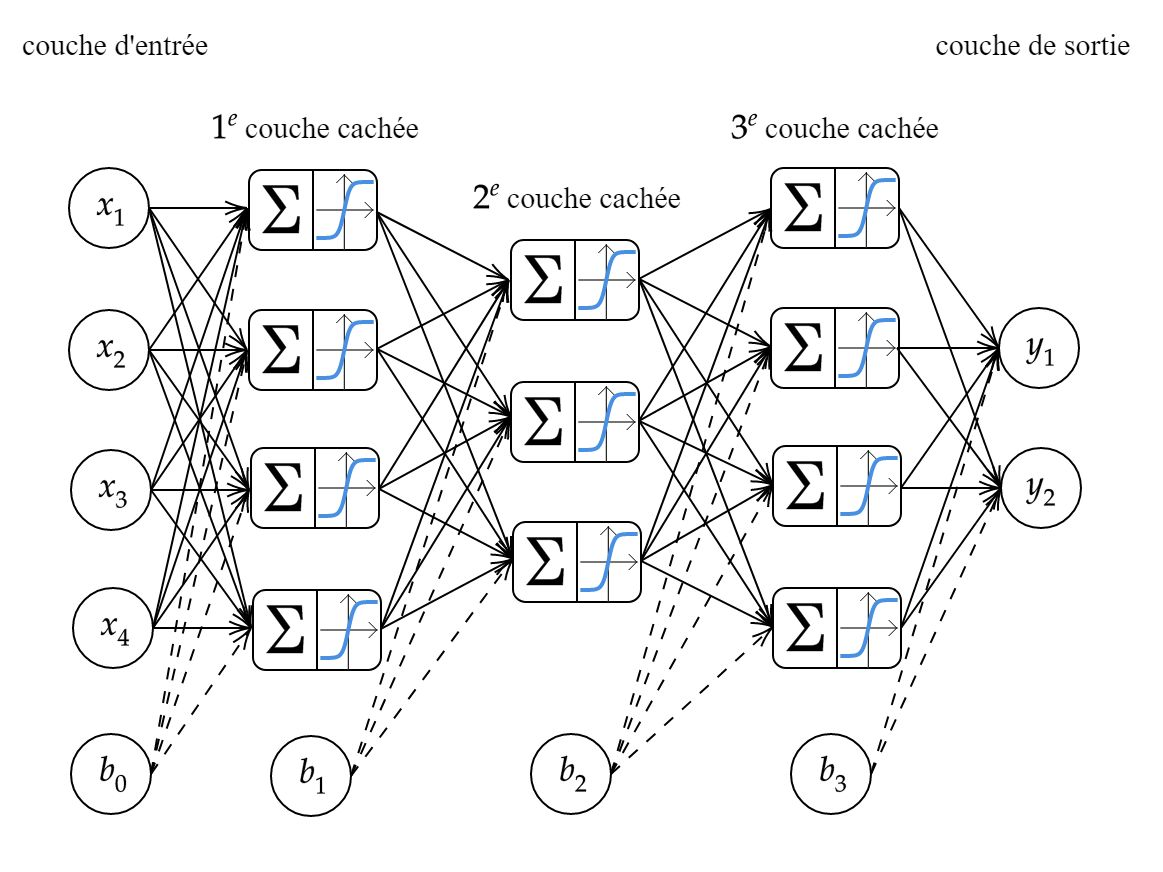
\includegraphics[width=0.85\linewidth]{figures/Chap2/perceptron-diagram.jpg}
  \centering
  \caption{\small{Exemple d'un perceptron multicouches avec 5 couches. }}
  \label{fig:reseau_neurones_artificiels}
\end{figure}

\subsection{Les réseaux de neurones à convolution}

L'architecture des \acrconvnet a été inspirée par les travaux de Hubel et Wiesel \cite{hubel1962receptive} sur le cortex visuel des mammifères.  Ils introduisirent la notion de champ récepteur d'un neurone du système visuel qui est la portion du champ visuel qui, lorsqu'on lui présente un stimulus lumineux, modifie la réponse de ce neurone.  Ils ont démontré que les neurones des premières couches du cortex visuel s'activaient en fonction de différents types de stimuli. Les neurones fonctionnaient comme des détecteurs simples, certains étaient spécialisés pour la détection de motifs linéaires dans un sens et certains autres groupes de neurones détectaient les motifs linéaires dans un autre sens. Les premiers algorithmes se rapprochant des \acrconvnet remontent aux années 1980 avec les travaux de Fukushima \cite{Fukushima1980} et le Neocognitron (Fig. ~\ref{fig:neocognitron-architecture-diagram}).  Le modèle introduit la notion d'une série de transformations hiérarchiques qui extraient des caractéristiques visuelles de plus en plus complexes pour déterminer la classe de sortie. %Cependant, le Néocognitron diffère des  \acrconvnet en ce que les poids des filtres ne sont pas partagés.

\begin{figure}[!htbp] 
  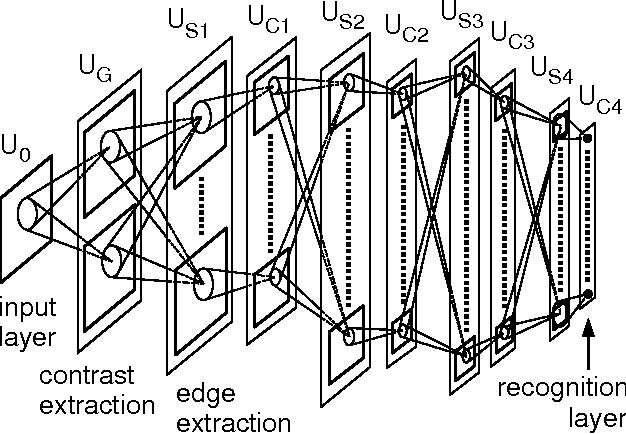
\includegraphics[width=0.60\linewidth]{figures/neocognitron.jpg}
  \centering
  \caption{\small{Architecture du Neocognitron \cite{Fukushima1980} }}
  \label{fig:neocognitron-architecture-diagram}
\end{figure}

\begin{figure}[!htbp] 
  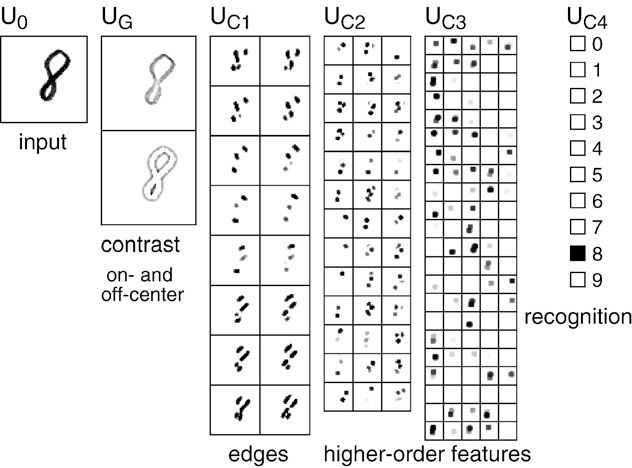
\includegraphics[width=0.60\linewidth]{figures/neocognitron2.jpg}
  \centering
      \caption%
            {{\small Un exemple des réponses de la sortie de chaque couche du Neocognitron. L'entrée est détectée correctement comme le chiffre 8. \cite{Fukushima1980}}}    
            \label{fig:neocognitron-outputs-diagram}
\end{figure}


Ce n’est que dans les années 1990, grâce aux travaux sur la reconnaissance des caractères manuscrits par LeCun et al  \cite{LeCun1998}, que les \acrconvnet seront popularisés. Les auteurs ont proposé une série d'architectures (\textbf{LeNet}) qui influencerons les recherches suivantes.  L'apprentissage des réseaux se font par rétropropagation du gradient de l'erreur. 

Plus formellement, dans le cas des \acrconvnetns, l'Équation \ref{eq:h_matricielle} transforme la multiplication matricielle des poids par une opération de convolution ($\ast$):

 \begin{equation}
     h = \varphi_i(W^\intercal  \ast x + b)
     \label{eq:h_convolution}
 \end{equation}
 
\vspace{10pt}

 La convolution est une opération mathématique sur deux fonctions (f et g) qui produit une troisième fonction exprimant la façon dont la forme de l'une est modifiée par l'autre:
 
\begin{equation}
    \begin{split}
        s(t) & = (f \ast g)(t) \\ 
             & = \int_{- \infty}^{\infty} f(a)\,g(t-a)\,da \\
             & = \sum_{a=- \infty}^{\infty} f(a)\,g(t-a) \\
             & = (g \ast f)(t) \\
             & = \sum_{a=- \infty}^{\infty} f(t-a)\,g(a)
   \end{split}
\end{equation}

\vspace{10pt}

Dans le cas des images, l'opération du convolution sur un signal en 2 dimensions est donnée par la double somme suivante:

\begin{equation}
    S(i,j) = (K \ast I)(i,j) = \sum_{m} \sum_{n} I(i+m, j+n)\,K(m,n)
    \label{eq:oper_conv}
\end{equation}

\vspace{10pt}

où $I$  représente notre image d'entrée et $K$ représente le noyau (filtre) de l'opération de convolution.  Lors de l'apprentissage d'un \acrconvnet les poids \textbf{W} de l'Équation \ref{eq:h_convolution} correspondent aux poids du filtre $K(m,n)$ de l'Équation \ref{eq:oper_conv}. La sortie $S(i,j)$ correspond à la carte de caractéristiques avant l'application de la fonction d'activation.

L'architecture des \acrconvnet s’appuie sur trois principes fondamentaux:

\begin{enumerate}
\item  Des champs récepteurs locaux associés à des convolutions (filtres, noyaux) qui permettent de détecter des caractéristiques visuelles élémentaires sur l’image, formant ainsi des cartes de caractéristiques;
\item  Le partage des poids, qui consiste à apprendre les mêmes poids d’une convolution et par le fait même d’extraire les mêmes types de caractéristiques visuelles pour toutes les positions sur l’image; 
\item  Des opérations de ré-échantillonnage (pooling) qui permettent de réduire la sensibilité aux translations, ainsi que de réduire le coût du traitement;
\end{enumerate}
Le deuxième principe présente la pierre angulaire des \acrconvnetns, car il permet de réduire considérablement la taille du réseau en mémoire et en diminuant le nombre de paramètres à apprendre. Cela permet à son tour de construire des architectures multicouches qui opèrent sur des entrées de grande dimension tout en demeurant de taille réaliste (ce qui est irréalisable avec les \acrmlpns). 

L’architecture typique des \acrconvnet (Fig. ~\ref{fig:convnet-lenet-diagram}) est composée par une séquence de plusieurs couches comprenant la couche d’entrée, quelques couches cachées et la couche de sortie.  Les couches cachées consistent en une ou plusieurs couches convolutives avec en sortie une fonction d’activation  qui utilise la somme pondérée de toutes les entrées de la couche précédente pour générer une valeur de sortie transformée par une fonction d'activation non-linéaire.  Cette valeur est transmise à la couche suivante. La fonction d'activation est quelquefois suivie d’une couche de re-échantillonage (\textit{pooling}) qui effectue une réduction de la sortie antérieure en prenant généralement la valeur maximale ou la valeur moyenne de l'ensemble d'une zone regroupée. Le réseau peut se terminer par une ou plusieurs couches entièrement connectées intercalées avec des couches d’activation non-linéaire. Les couches convolutives effectuent des calculs locaux définis par la taille des champs réceptifs et les couches entièrement connectées apprennent les représentations globales de l'image sur toutes les activations des couches précédentes. 

\begin{figure}[!htbp] 
  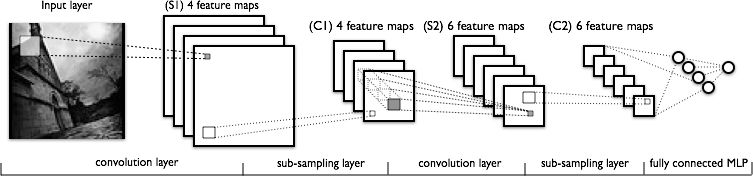
\includegraphics[width=\linewidth]{figures/convnet-lenet-diagram.jpg}
   \caption{\small{Architecture d'un réseau \textbf{LeNet} démontrant les structures de base des \acrconvnet}}
  \label{fig:convnet-lenet-diagram}
\end{figure}

Pendant l’opération de convolution, les filtres de la taille du champ récepteur local sont convolués avec l’image pour produire une valeur de sortie pour chaque pixel, formant des cartes de caractéristiques pour chaque filtre.  Ces cartes deviennent à leur tour l’entrée de la prochaine couche convolutive et produisent d’autres cartes de caractéristiques.  Ce procédé hiérarchique est répété en séquence pour toute la pile de couches convolutives (Fig. \ref{fig:convolution-diagram}).

\begin{figure}[!htbp] 
  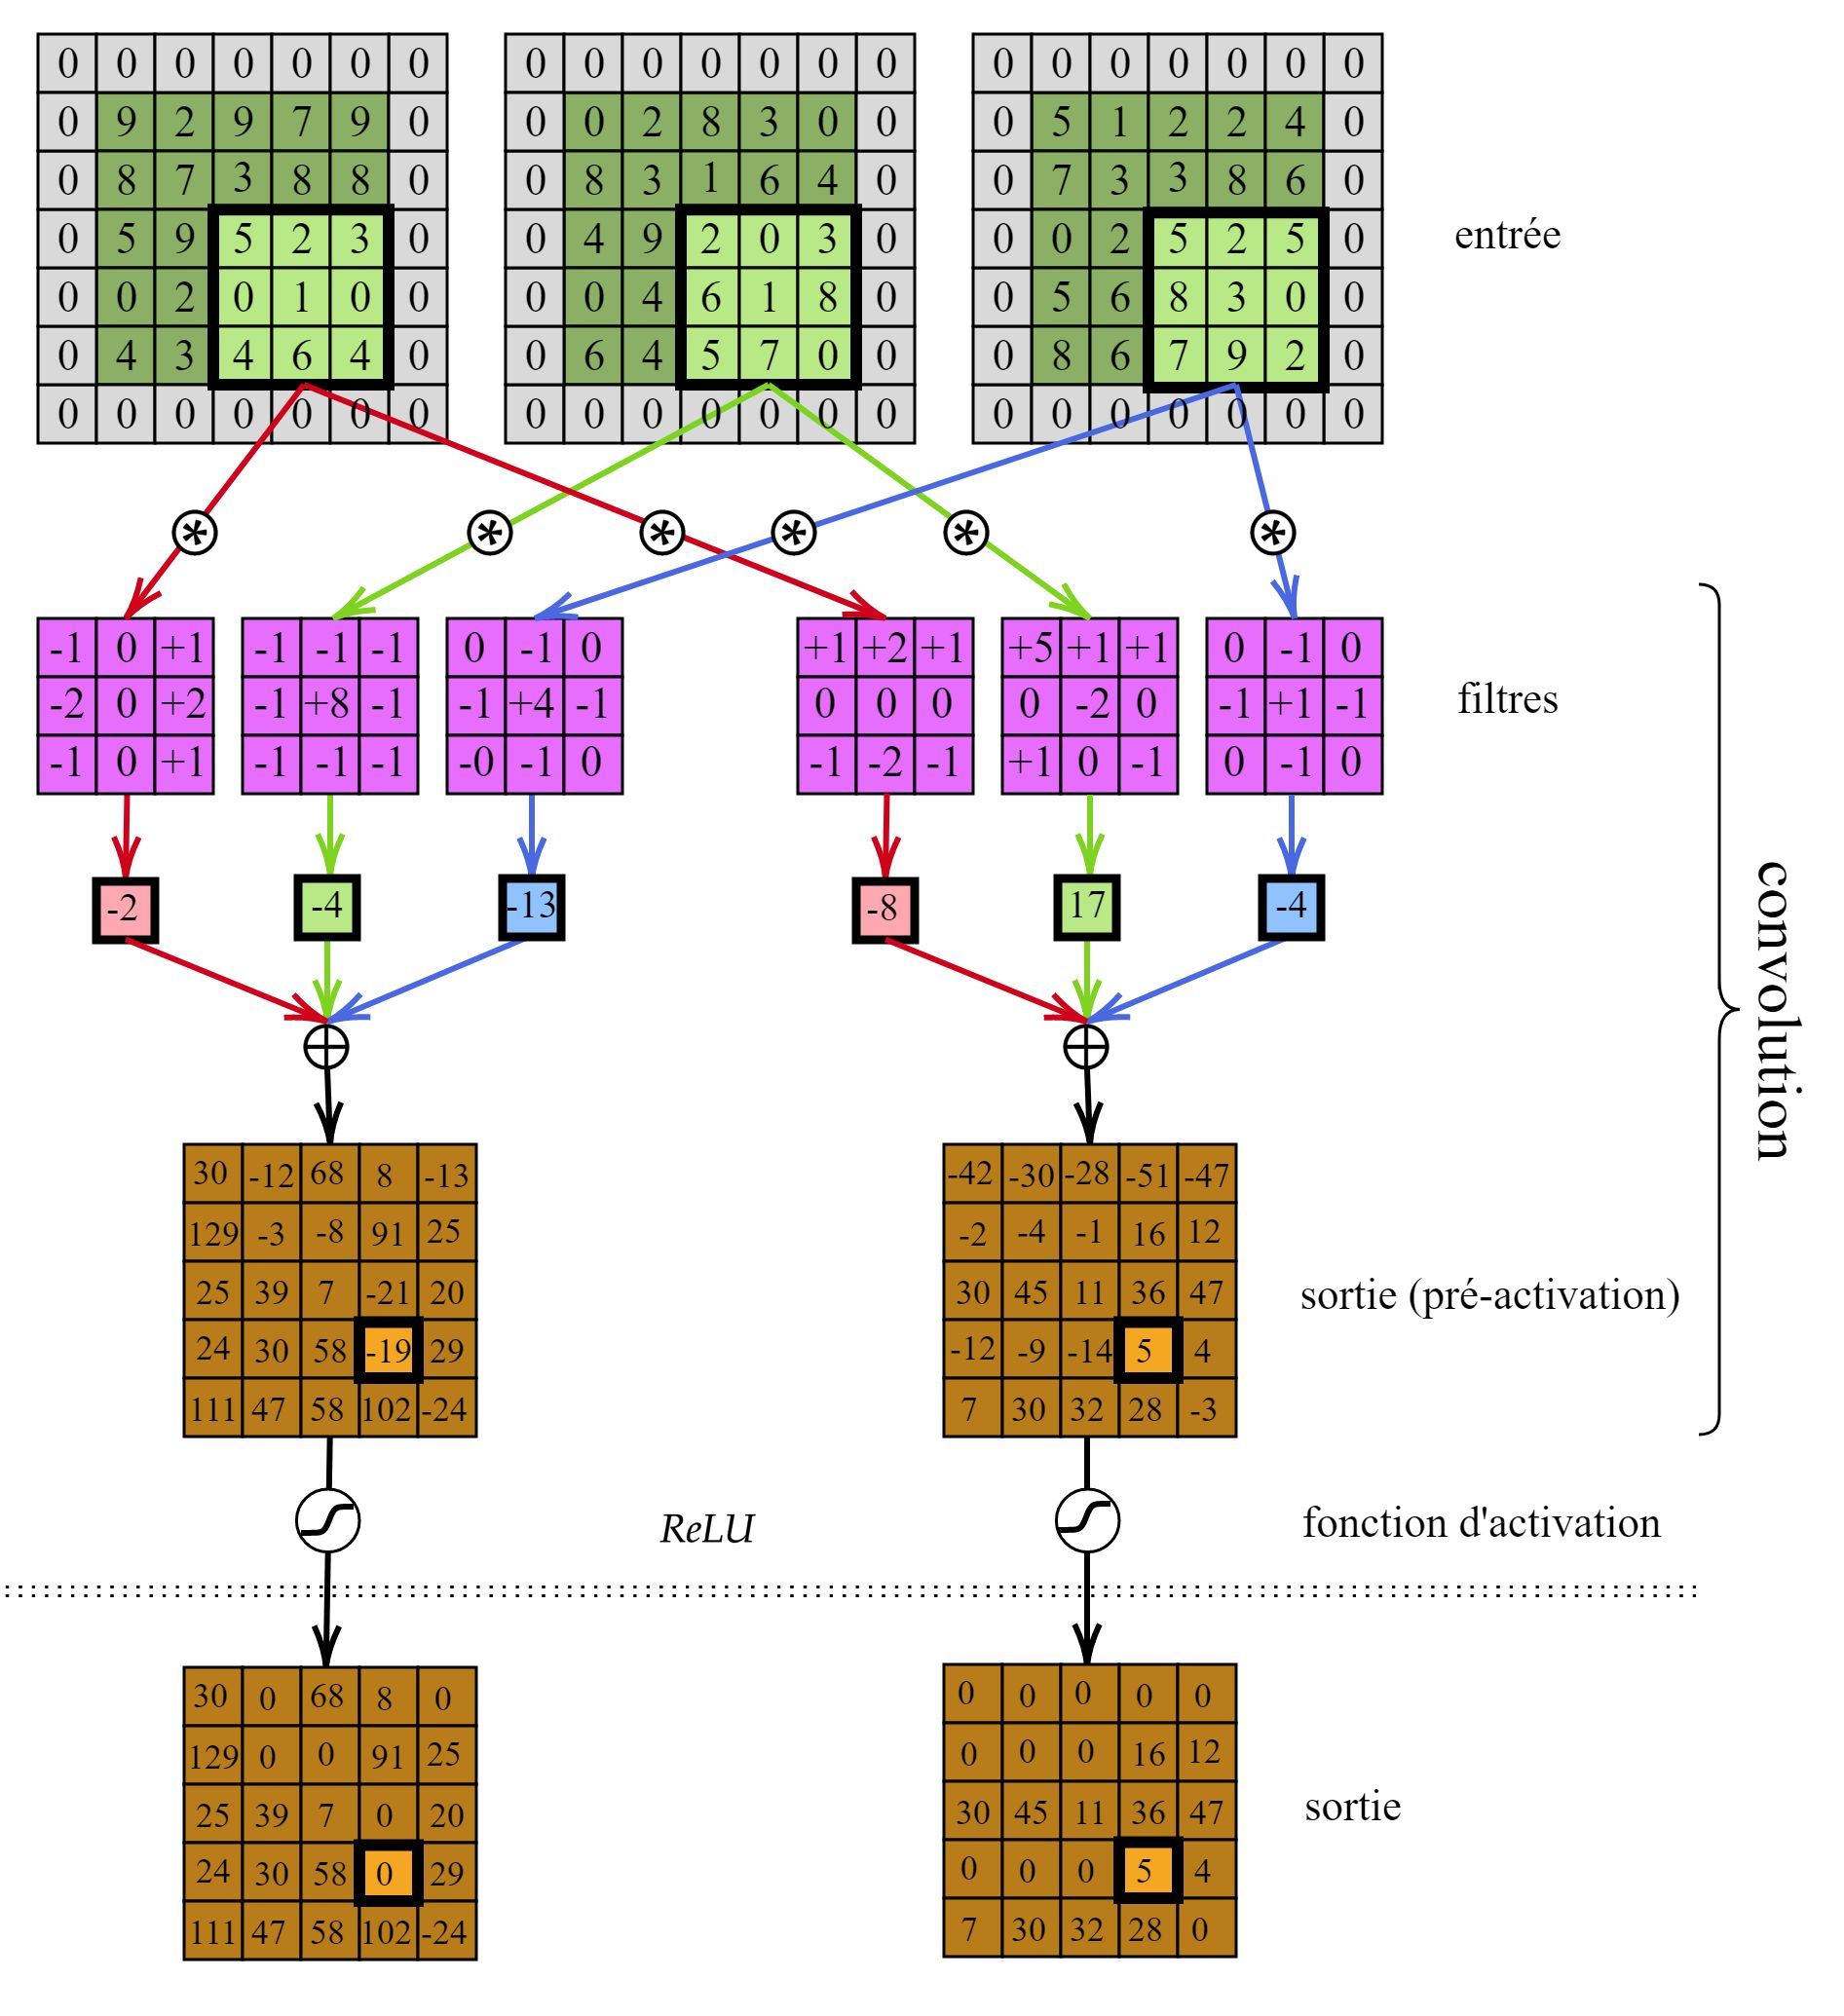
\includegraphics[width=0.95 \linewidth]{figures/Chap2/convolution-diagram.jpg}
   \centering
\caption
{\small Illustration des opérations d'un bloc convolutif $conv+ReLU$.}
  \label{fig:convolution-diagram}
\end{figure}

La fonction d’activation est appliquée aux cartes de caractéristiques.  Cette fonction peut être une des très nombreuses fonctions non-linéaires existantes, soient entre autres l’unité de rectification linéaire (\textbf{ReLU}) \cite{Glorot2011}, la fonction tangente hyperbolique ou la fonction sigmoïde (Fig. \ref{fig:activation-functions-diagrams}). 

\begin{figure}[!htbp] 
  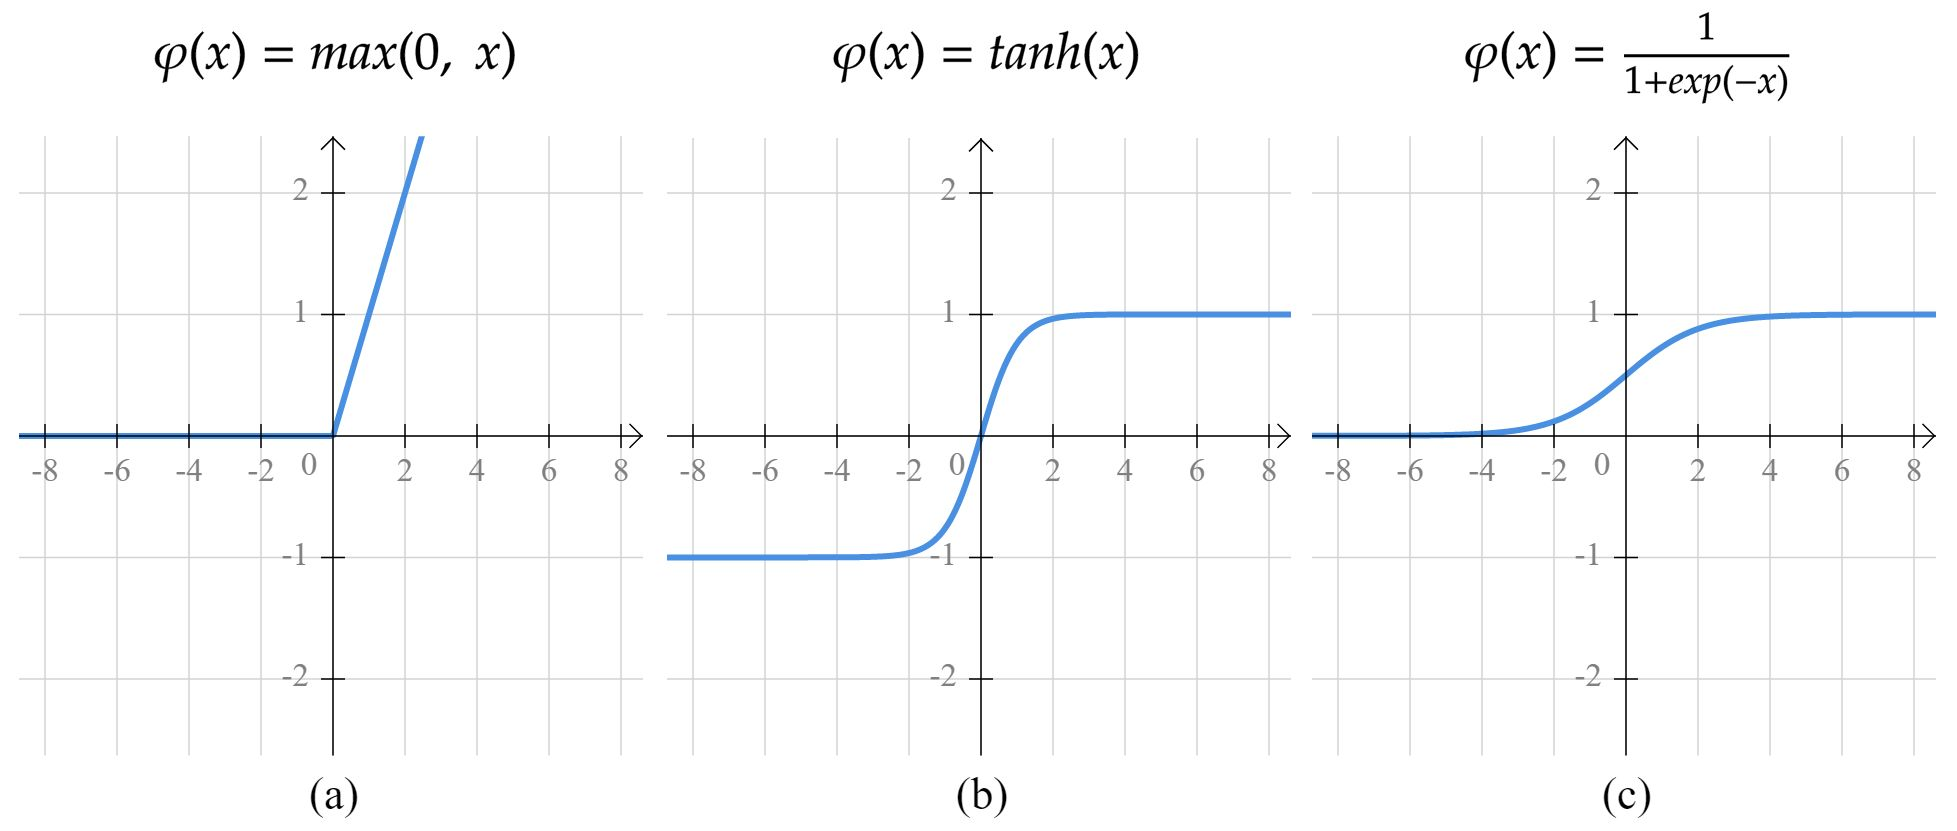
\includegraphics[width=0.75 \linewidth]{figures/Chap2/activation-functions-diagram.jpg}
   \centering
\caption
{\small Illustration de certaines fonctions d'activation non-linéaires. (a) Rectifier Linear Unit (ReLU), (b) tangente hyperbolique, (c) sigmoïde}
  \label{fig:activation-functions-diagrams}
\end{figure}

La couche d'échantillonage de type \textit{max} sélectionne la valeur maximale des éléments des cartes de caractéristiques dans un voisinage de taille définie, tandis la couche d'échantillonage de type \textit{ave} sélectionne la valeur moyenne.  Dans le cas où le ré-échantillanage est appliqué avec un pas égal ou supérieur à la taille du voisinage, les cartes de caractéristiques seront sous-échantillonnées, de sorte que les prochaines étapes d’analyse seront effectuées à plus large échelle avec une résolution diminuée.  L’application de la couche de ré-échantillonage a pour objectif premier d’augmenter la robustesse du \acrconvnet au bruit et  aux distorsions spatiales.  De plus, en réduisant la taille du réseau, on bénéficie d’une réduction du nombre de paramètres à estimer et du risque de surapprentissage.

\begin{figure}[!htbp] 
  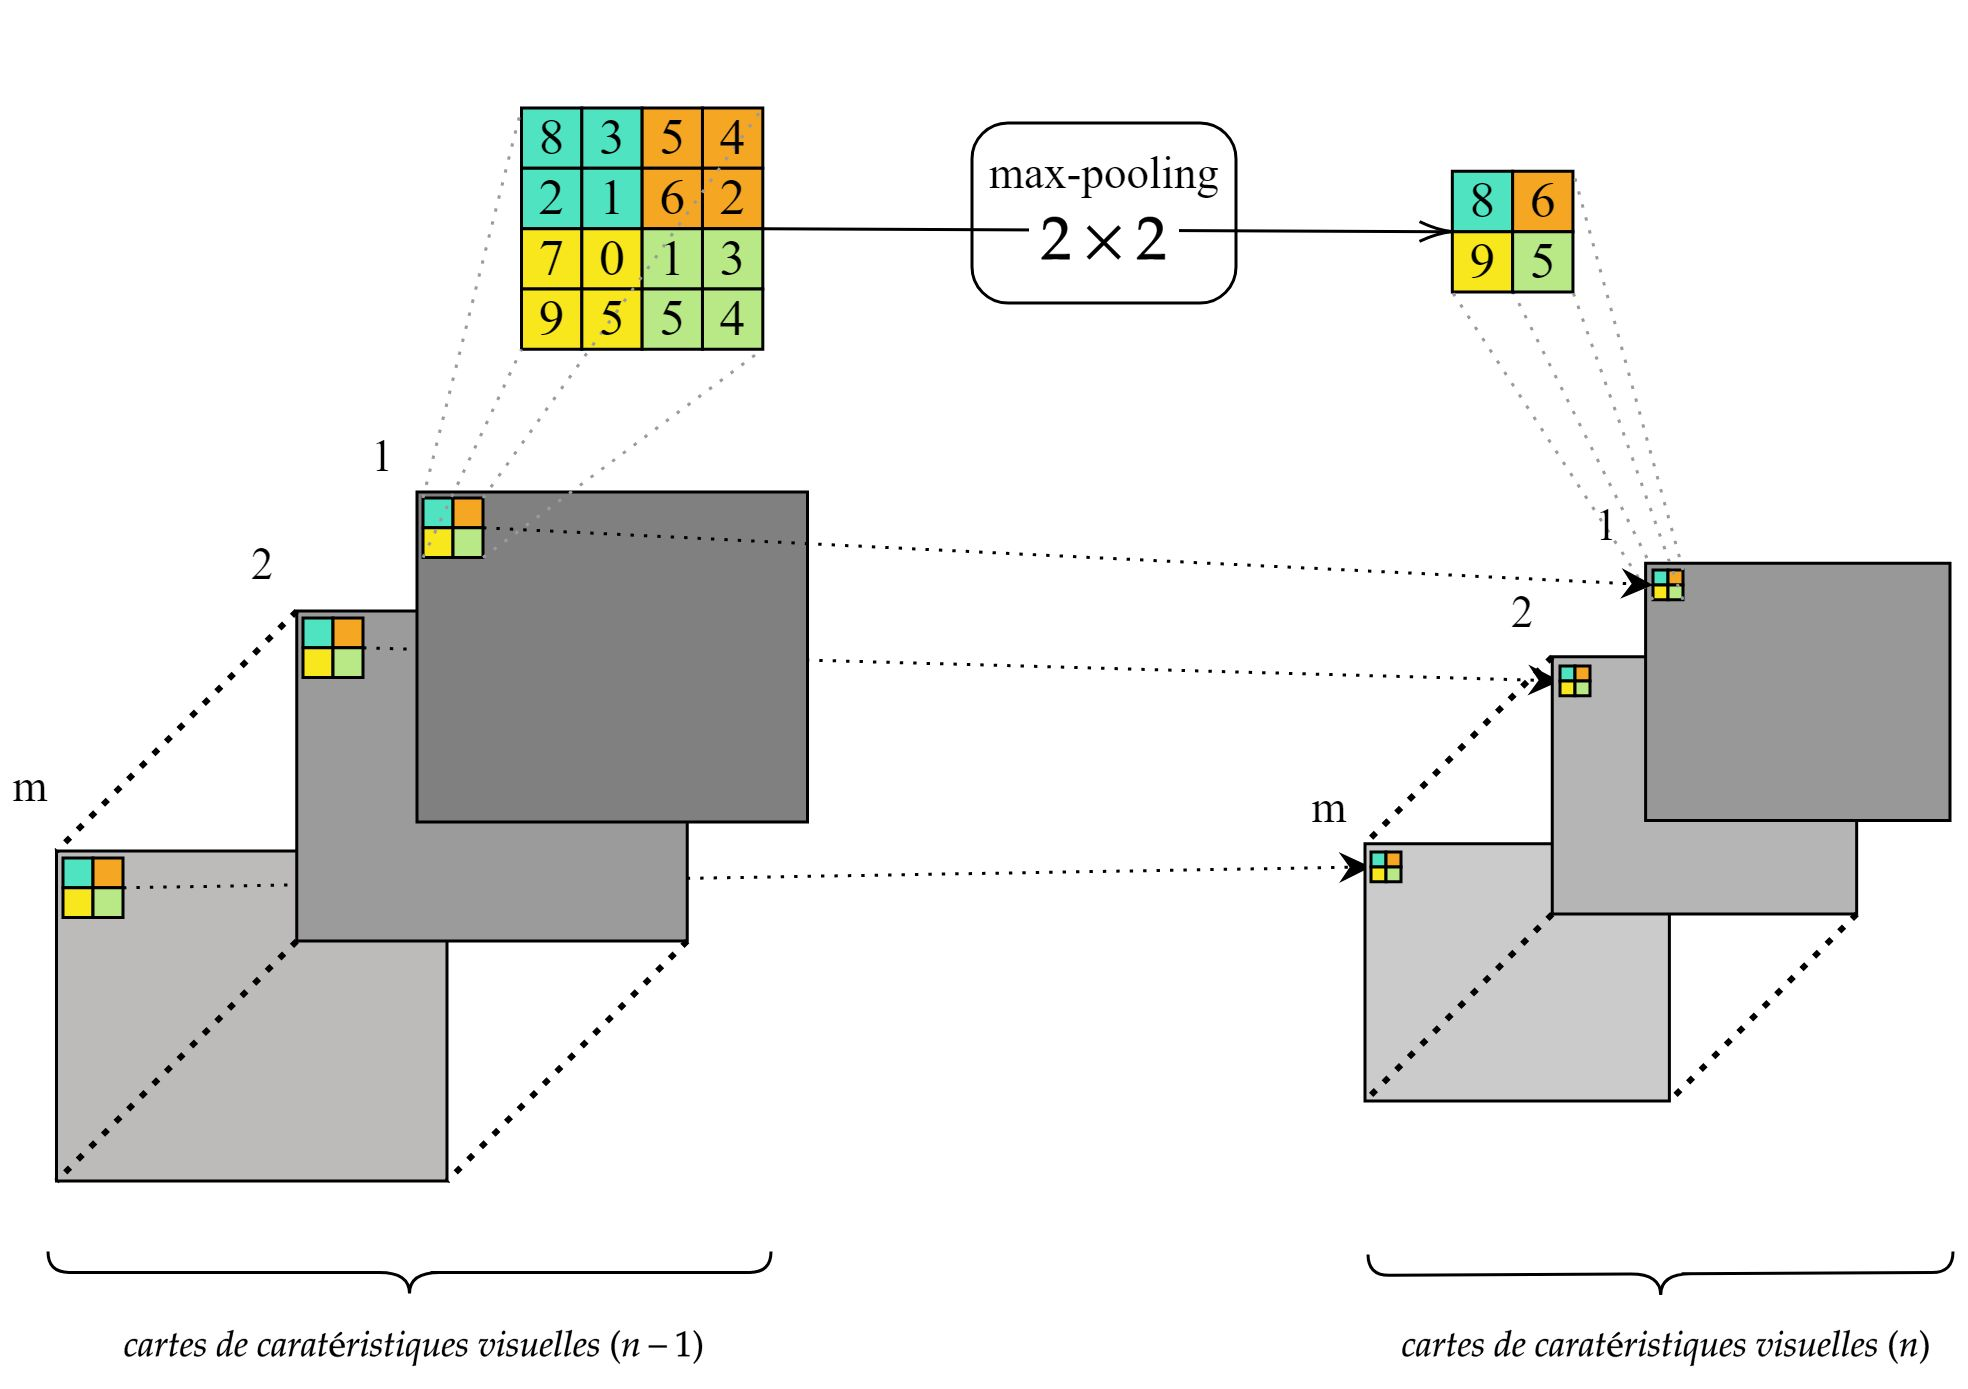
\includegraphics[width=0.75 \linewidth]{figures/Chap2/max-pooling-diagram.jpg}
   \centering
\caption
{\small Illustration de l'opération d'échantillonage \textit{max-pooling}}
  \label{fig:max-pooling-diagram}
\end{figure}

La sortie de la dernière couche convolutive est applatie pour être injectée dans les couches entièrement connectées. Ces couches sont complètement connectées en amont comme en aval, impliquant un nombre élevé de paramètres à estimer si on les compare aux couches convolutives. Ce genre de configuration a été couramment utilisé avec succès pour la classification en vision par ordinateur. Les modèles de classification les plus reconnus mettant en œuvre cette configuration sont les gagnants successifs du concours ILSVRC: AlexNet (2012) \cite{Krizhevsky2012}, ZFNet (2013) \cite{ZFNet}, VGGNet (2014, $2\ts{e}$ position)  \cite{vgg}, GoogLeNet (2014) \cite{Szegedy2015} et ResNet (2015) \cite{He2015DelvingDI}.

Les réseaux à résidus (ResNet) (He et all. \cite{He2015DelvingDI}) ont introduit une composante importante dans l’architecture des \acrconvnetns.  Ces réseaux ont des connections de saut qui permettent au signal original $x$ de traverser comme suit les couches: $G(x)=F(x)+x$. Ils forment des blocs résiduels (Fig. ~\ref{fig:resnet-block-diagram}).  La fonction $F(x)$ apprend le résiduel, qui est la différence entre le résultat final et le signal d’entrée $x$. L'effet de ce saut de connections est de limiter le problème du gradient évanescent que l'on rencontre parfois lors de l'apprentissage de réseaux neuronaux avec la méthode de rétropropagation du gradient de l'erreur. 

\begin{figure}[!htbp] 
  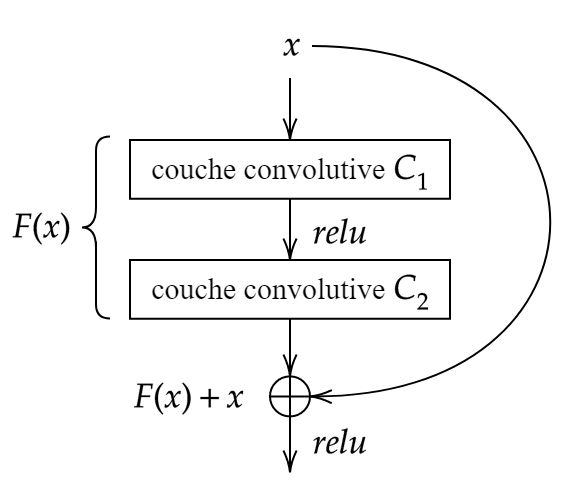
\includegraphics[width=0.30\linewidth]{figures/resnet-block-diagram.jpg}
   \caption{\small{Illustration d'un bloc résiduel}}
  \label{fig:resnet-block-diagram}
\end{figure}

\subsection{Les réseaux de neurones pleinement convolutifs}

Les réseaux de neurones pleinement convolutifs (\acrfcnns) (\textit{fully convolutional network}) sont utilisés pour la segmentation sémantique (Shelhamer et al.\cite{Shelhamer2017}), l'étiquetage de scène (Pinheiro et all. \cite{Pinheiro2013RecurrentCN}) et pour la détection de caractéristiques (Sermanet et al. \cite{Sermanet2013OverFeatIR}). En télédétection, Sherrah \cite{Sherrah2016FullyCN} a obtenu des résultats de pointe avec les \acrfcn pour l'étiquetage sémantique des images aériennes. 

L’architecture (\acrfcnns) est semblable à celle des \acrconvnet à la différence que les couches entièrement connectées sont omises. La dernière couche est directement connectée à la fonction de perte pour l’apprentissage. Cette omission de la partie \acrmlp change le fonctionnement du réseau de trois façons: 
\begin{enumerate}
    \item La couche \acrmlp permet au réseau d’apprendre des représentations globales dans lesquelles les relations spatiales des cartes de caractéristiques sont ignorées. Ce n'est plus le cas avec les \acrfcn où le réseau tente d'apprendre des représentations qui tiennent compte  des relations spatiales locales;
     \item Les \acrfcn peuvent recevoir des entrées de taille arbitraire, contrairement aux \acrconvnet qui n’acceptent que des entrées de taille fixe;
    \item Les \acrconvnet retournent une seule valeur, les \acrfcn produisent des cartes de sortie grossières lorsqu'un ré-échantillonnage est appliqué;
\end{enumerate}
Pour reconstruire la résolution originale de l’image deux approches sont proposées. Sherrah \cite{Sherrah2016FullyCN} suggère une approche “\textit{shift and stitch}” où les cartes grossières calculées par translation de la position sur l’image d’entrée sont fusionnées pour former une carte dense.  La seconde approche consiste à utiliser des couches déconvolutives (Zeiler et al. \cite{Zeiler10deconvolutionalnetworks}) après toutes les couches convolutives pour suréchantillonner la sortie sous-échantillonnée afin d'obtenir la couche de sortie finale (Fig. \ref{fig:conv-deconv-block-diagram}).

\begin{figure}[!htbp] 
  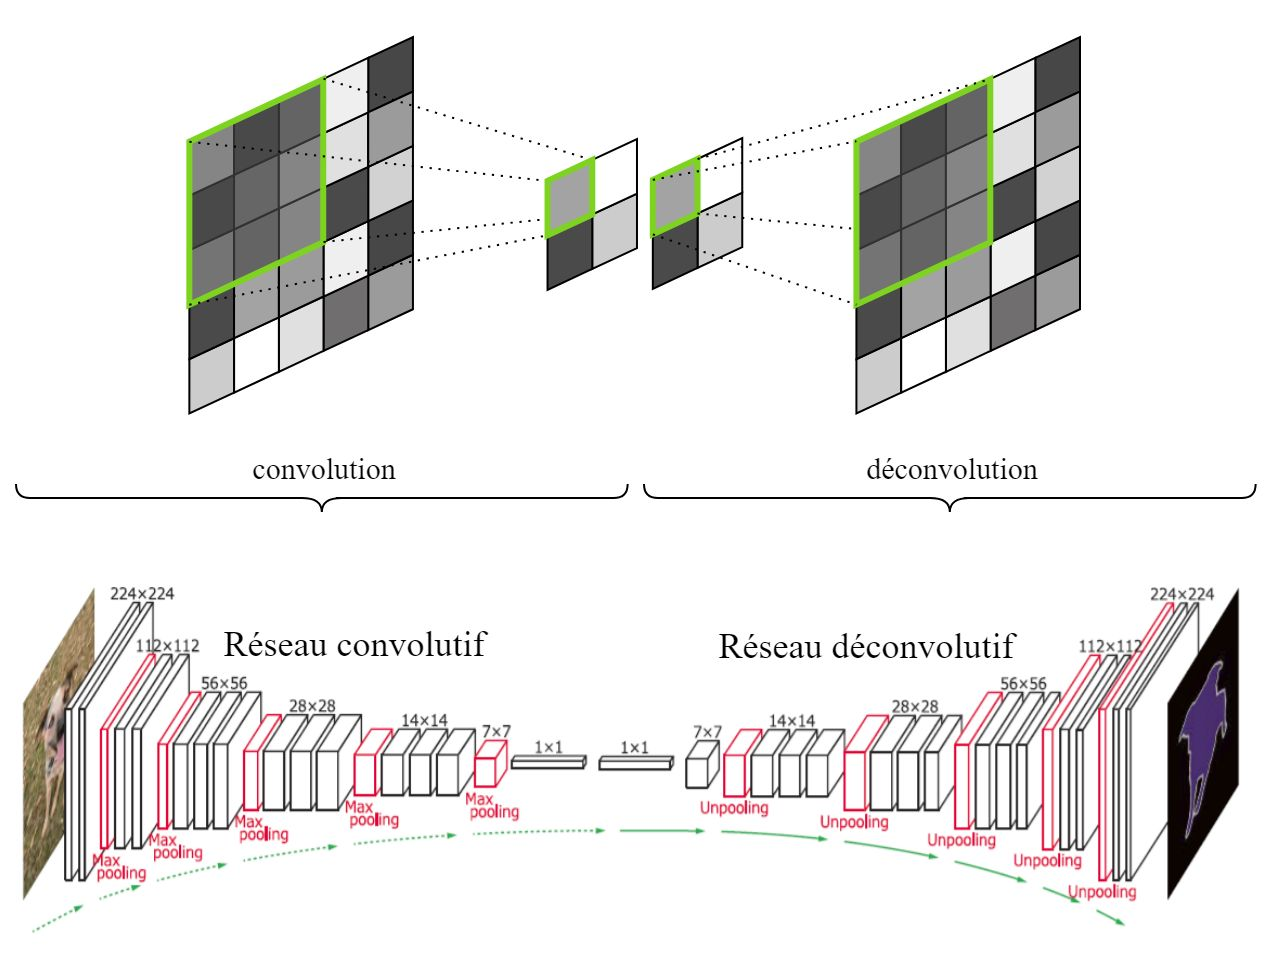
\includegraphics[width=0.85\linewidth]{figures/deconvolution.jpg}
   \caption{\small{Illustration de l'opération convolution versus l'opération déconvolution}}
  \label{fig:conv-deconv-block-diagram}
\end{figure}

Une autre architecture \acrfcn que l’on retrouve surtout en restauration d’image est un réseau formé purement de couches convolutives et de couches d’activation (Fig. ~\ref{fig:convnet-vdsr-diagram}).  Ces réseaux produisent en sortie une carte de caractéristiques (\textit{features map}) de la même dimension que la taille 2D de l’entrée. Le nombre de canaux formant la sortie dépend du nombre de convolutions de la dernière couche.  Le champ réceptif de la couche d'entrée est généralement plus petit, car sans cela le nombre de paramètres à apprendre serait trop grand. Le réseau se termine habituellement par une fonction de perte qui calcule une régression.  Ce genre de configuration a été couramment utilisé avec succès pour les problèmes de superrésolution (Dong et al. \cite{Dong2016}; Kim et al. \cite{Kim2016}), débruitage en général (Zhang et al. \cite{Zhang2017}, \cite{Zhang2018}).  Dans le cadre de ce mémoire, nous utiliserons cette approche pour calculer nos modèles pour le filtrage du chatoiement.

\begin{figure}[!htbp] 
  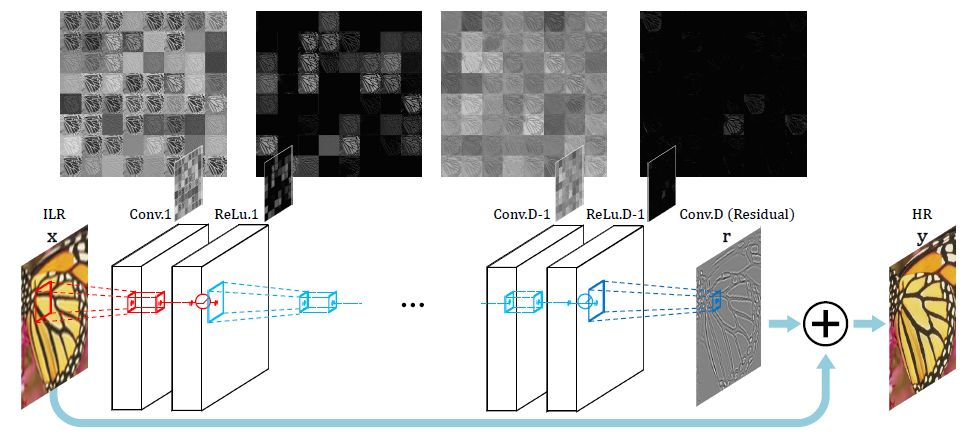
\includegraphics[width=\linewidth]{figures/vdsr-diagram.jpg}
   \caption{\small{Exemple d'un \acrfcn sans couche de ré-échantillonage utilisé en superrésolution: VDSR (\textit{Very Deep Super Resolution} \cite{Kim2016} ).  }}
  \label{fig:convnet-vdsr-diagram}
\end{figure}

\section{L'apprentissage des réseaux}

Les approches en apprentissage machine profond utilisent plusieurs techniques issues de l'apprentissage machine en générale.  Nous décrivons dans cette section certaines techniques que nous utiliserons. Les grandes étapes du fonctionnement d'un apprentissage sont décrites par l'Algorithme \ref{alg:basic_machine_learning_steps}. Considérons un ensemble de données $(X, y)$ où $X$ est la donnée caractéristique et $y$ est son étiquette.  Un modèle $F(\Theta, X)$ permet de calculer un estimé $\bar{y} = F(x)$. Les valeurs $\Theta$ sont les paramètres du modèle.  L'objectif de l'apprentissage est de trouver les paramètres qui minimisent l'erreur $\epsilon$ entre l'estimé $\bar{y}$ et l'étiquette $y$. La minimisation se fait en trouvant les minimums de la fonction $\epsilon$, ce qui implique que cette dernière doit être convexe.

\begin{algorithm}[]
\small
\SetAlgoLined
 Initialiser le modèle avec des poids aléatoires;
 
 \PourCh{exemple de la liste des données d'entraînement}{
    \begin{enumerate}
     \item Donner l'entrée au modèle pour obtenir la sortie; 
     \item Calculer l'erreur en comparant la sortie avec le résultat cible
     \item Propager l'erreur de couche en couche vers l'arrière
     \item Mettre à jour tous les poids du réseau
 \end{enumerate}
 }
 \caption{Étapes générales de l'apprentissage d'un réseau de neurone}
 \label{alg:basic_machine_learning_steps}
\end{algorithm}

\subsection{Optimisation par descente du gradient}

L'optimisation par descente du gradient est un algorithme d'optimisation de premier ordre.  Il permet de calculer les minimum locaux d'une fonction de coût convexe à partir des dérivées premières. La descente de gradient ajuste de manière itérative les paramètres du modèle afin de trouver progressivement la meilleure combinaison de poids et de biais pour minimiser la fonction de coût en fonction des données d'apprentissage.  La mise à jour des paramètres est fait selon:

\begin{equation}
      \Theta = \Theta - \lambda \cdot \frac{1}{N} \sum_{n=1}^{N} \frac{\partial \epsilon(y, \bar{y})}{\partial \Theta}
      \label{eq:gradient_descent}
\end{equation}

où $\lambda$ est le taux d'apprentissage.  La valeur $\lambda$ règle la vitesse de la mise à jour des paramètres. L'Algorithme \ref{alg:sgd} présente le pseudo-code de la méthode.
\newline

\begin{algorithm}[]
\small
\SetAlgoLined
\Sortie{ Paramètres $\Theta$ optimaux qui minimisent $\epsilon$ }
\Entree{Fonction de coût $\epsilon$; Taux d'apprentissage $\lambda$; Ensemble de données $(X, y)$; Modèle $F(\Theta, x)$}

initialisation aléatoire des paramètres $\Theta$\; 
 \Tq{La minimisation converge?}{
 
 \begin{enumerate}
     \item Calculer la prédiction $\bar{y}$\; 
     $\bar{y} = F(\Theta, x)$
     \item Ajuster les paramètres $\Theta$\; 
     $\Theta = \Theta - \lambda \cdot \frac{1}{N} \sum_{n=1}^{N} \frac{\partial \epsilon(y, \bar{y})}{\partial \Theta}$
 \end{enumerate}
  
 }
 \caption{La descente du gradient}
  \label{alg:sgd}
\end{algorithm}

\subsection{Optimisation par descente du gradient stochastique par mini-lots}

L'algorithme de descente de gradient par mini-lots estime le gradient à partir d'un petit sous-ensemble des données d'apprentissage $x_i, y_i \in (X,y)$.  Il permet d'accélérer l'apprentissage. La version \textit{Vanilla} utilise un mini-lot de taille 1. Dans la plupart des cas, l'algorithme de la descente de gradient peut trouver un point proche du minimum d'une fonction strictement convexe. Dans le cas de la descente de gradient stochastique par mini-lots, il n'est pas garanti de trouver ce point mais une forte probabilité. A noter que les modèles profonds ne sont jamais des fonctions convexes. Cependant les algorithmes conçus pour l'optimisation convexe trouvent généralement des solutions suffisamment satisfaisantes pour les réseaux profonds, mais ils ne garantissent pas que les solutions soient des minimums globaux. L'Algorithme \ref{alg:sgd_mini_batches} présente le pseudo-code de la méthode.

\begin{algorithm}[]
\small
\SetAlgoLined
\Sortie{ Paramètres $\Theta$ optimaux qui minimisent $\epsilon$ }
\Entree{Fonction de coût $\epsilon$; Taux d'apprentissage $\lambda$; Ensemble de données $(X, y)$; Modèle $F(\Theta, x)$}.
 initialisation aléatoire des paramètres $\Theta$\; 
 
 \Tq{La minimisation converge?}{
 
 Mélanger l'ensemble $(X, y)$\;
 
 \PourCh{mini-lot $x_i, y_i \in (X, y)$}{
 \begin{enumerate}
     \item Calculer la prédiction $\bar{y}$\; 
     $\bar{y_i} = F(\Theta, x_i)$
     \item Ajuster les paramètres $\Theta$\; 
     $\Theta = \Theta - \lambda \cdot \frac{1}{N} \sum_{n=1}^{N} \frac{\partial \epsilon(y_i, \bar{y_i})}{\partial \Theta}$
 \end{enumerate}

 }
 }
 \caption{La descente du gradient par mini-lots}
   \label{alg:sgd_mini_batches}
\end{algorithm}

\subsection{Optimisation par rétropropagation du gradient de l'erreur}

La rétropropagation du gradient de l'erreur est employée pour calculer la descente de gradient sur des réseaux de neurones. La méthode calcule le gradient de l'erreur en fonction des paramètres du réseaux de manière récursive de la couche de sortie jusqu'à la première couche afin d'optimiser les paramètres.  L'Algorithme \ref{alg:backpropagation} présente le pseudo-code de la méthode.

% https://google-developers.appspot.com/machine-learning/crash-course/backprop-scroll/?hl=FR

\begin{algorithm}[]
\small
\SetAlgoLined
\Entree{Un réseau de neurones avec j couches; La fonction d'activation $\varphi_j(\cdot)$; Les sorties des couches cachées $h_j=\varphi_j(W_j^T \cdot h_{j-1}+b_j)$; et la sortie du réseau $\bar{y}=h_j$.
}
 Calculer le gradient de la couche de sortie: $\delta 	\leftarrow \frac{\partial \epsilon(y, \bar{y})}{\partial y}$ 
 
 \Pour{$i \leftarrow j$ à 1}{
 
 \begin{enumerate}
   \item Calculer le gradient de la couche courante pour les poids et les biais:
   
     $\frac{\partial \epsilon (y, \bar{y})}{\partial W_j} = \frac{\partial \epsilon (y, \bar{y})}{\partial h_j} \frac{\partial h_l}{\partial W_j} = \delta \frac{\partial h_l}{\partial W_j}  $
     
      $\frac{\partial \epsilon (y, \bar{y})}{\partial b_j} = \frac{\partial  \epsilon (y, \bar{y})}{\partial h_j} \frac{\partial h_l}{\partial b_j} = \delta \frac{\partial h_l}{\partial b_j}  $
    \item Appliquer l'algorithme de la descente du gradient:
    
    $W_j \leftarrow W_j - \lambda \frac{\partial \epsilon (y, \bar{y})}{\partial W_j}$
    
      $b_j \leftarrow b_j - \lambda \frac{\partial \epsilon (y, \bar{y})}{\partial b_j}$
      
     \item Rétropropager le gradient à la couche supérieure $j-1$:
     
     $\delta \leftarrow \frac{\partial \epsilon (y, \bar{y})}{\partial h_j} \frac{\partial h_l}{\partial h_{j-1}} = \delta \frac{\partial h_l}{\partial h_{j-1}} $  
  
 \end{enumerate}
  
 }
 \caption{La rétropropagation du gradient de l'erreur}
    \label{alg:backpropagation}
\end{algorithm}

